\documentclass{article}
\usepackage[utf8]{inputenc}
\usepackage{typearea}
\usepackage{multirow}
\usepackage{color, colortbl}
\usepackage{caption}
\usepackage{subcaption}
\usepackage{graphicx}
\usepackage{float}
\usepackage{lipsum}
\usepackage[pdftex]{hyperref}
\definecolor{Gray}{RGB}{231, 230, 230}

\tolerance=1
\emergencystretch=\maxdimen
\hyphenpenalty=10000
\hbadness=10000

\title{Exercício 4 - Precondicionadores e Reordenamento}
\author{Lorena B. Bassani}
\date{2021}

\begin{document}

\maketitle

\begin{abstract}
    Este documento relata os resultados do terceiro exercício da disciplina de Algoritmos Numéricos II, no semestre 2021/01 EARTE. O objetivo é observar o comportamento do Método dos Gradientes Conjugados e GMRES para um conjunto de matrizes esparsas da \textit{SuiteSparse Matrix Collection}\footnote{\href{https://sparse.tamu.edu}{https://sparse.tamu.edu}} considerarando precondicionamento e reordenamento.
\end{abstract}

\section{Introdução}
Para a primeira etapa deste exercício, foram utilizadas quatro matrizes quadradas esparsas, a \textit{mesh3em5} de $289$ linhas e colunas, a \textit{662\_bus} com $662$, a \textit{pdb1HYS} com $36.417$ e a \textit{Dubcova3} de dimensão $146.689$, e para a segunda etapa, foram utilizadas três matrizes quadradas esparsas, a \textit{cavity05} com $1.182$ linhas e colunas, a \textit{cz2548} com $2.548$ e a \textit{epb3} de dimensão $84.617$, obtidas da coleção de matrizes esparsas \textit{SuiteSparse Matrix Collection}. Nessas sete matrizes, foram realizadas análises quanto ao comportamento da aplicação de diferentes precondicionadores, com e sem reordenamento, utilizando a ferramenta Octave. Na seção~\ref{sec:resultados} são relatadas algumas observações sobre a utilização deste método para resolução de sistemas lineares, e na última parte do trabalho, nas seções~\ref{sec:figures} e~\ref{sec:tabelas}, se encontram as figuras e as tabelas com os resultados obtidos, respectivamente.

\section{Exercício Proposto -- Precondicionadores e Reordenamento}
\label{sec:resultados}
O objetivo deste exercício é observar o comportamento de matrizes esparsas na solução de sistemas lineares via métodos iterativos não estacionários, considerando precondicionamento e reordenamento. Para isto, as matrizes escolhidas foram submetidas a métodos de precondicionamento e reordenamento e utilizadas como matriz de coeficientes para solução de sistemas lineares através de método nativo do Octave, e foram observados uma série de fatores quanto ao comportamento das matrizes a respeito da convergência da resposta e seu número de condicionamento.

\subsection{Fatoração Incompleta de Cholesky -- ICC}

Na primeira parte do exercício, foi estudado o método da fatoração incompleta de Cholesky-ICC. Para isto, cada uma das quatro primeiras matrizes eram submetidas a duas configurações diferentes do método: a fatoração ICC(0), ou \textit{incomplete Cholesky with zero-fill}\footnote{De acordo com a documentação do método Octave ichol, disponível em: \href{https://octave.sourceforge.io/octave/function/ichol.html}{https://octave.sourceforge.io/octave/function/ichol.html}}, e a fatoração \textit{incomplete Cholesky with threshold dropping}. Cada uma foi realizada com e sem reordenamento. O resultado foi testado aplicando-o como entrada para o método dos gradientes conjugados, estudado no Exercício 2.

O método dos gradientes conjugados é um dos métodos que levariam a uma resposta exata em $n$ passos, a menos de erros de arredondamento, porém, levando em consideração que a maior parte do decrescimento do erro ocorre nos passos primários, ele é tratado como método iterativo, parando após atingir critérios de tolerância do erro. Isso faz com que o método, para matrizes bem condicionadas, convirja rapidamente, em pouquíssimas iterações quando comparado a dimensão da própria matriz. A ideia do uso de precondicionadores é melhorar o condicionamento da matriz de entrada, para melhorar a convergência do método.

Um dos passos realizados nas duas menores matrizes para verificar a diferença entre a matriz original e a matriz resultante do precondicionamento foi calcular o número de condicionamento delas\footnote{As matrizes \textit{pdb1HYS} e \textit{Dubcova3} não permitiram o calculo do número de condicionamento por serem muito grandes, causando fechamento forçado do programa Octave depois de certo tempo do início da operação. A operação de cálculo de condicionamento é tão ou até mais custosa do que a própria solução do sistema linear, podendo até não ser possível em alguns casos, como observado.}. Na \textit{mesh3em5}, o precondicionamento não alterou o número de condicionamento de forma significativa, de forma que este permaneceu o mesmo até as primeiras quatro casas decimais. O número de condicionamento dessa matriz ficou, assim, próximo de $4,9659$ tanto na original quanto nas precondicionadas. Já na matriz \textit{662\_bus}, o método de precondicionamento diminuiu o número de precondicionamento, levando de $7,941\times 10^5$ para seu menor número em $5,903\times 10^3$ com o precondicionamento ICC(0) sem reordenamento.

Outras observações realizadas antes de submeter as matrizes ao método dos gradientes conjugados foi a alteração do número de elementos não nulos. A matriz \textit{mesh3em5} possuía originalmente $1.377$ elementos não nulos, atingindo um máximo de $1.891$ com o precondicionamento ICC(0) sem reordenamento, e um mínimo de 833 no ICC, tanto com quanto sem reordenamento. Na matriz \textit{662\_bus}, que tinha originalmente $2.474$ elementos não nulos, encontrou um máximo de $5.910$ no precondicionamento ICC sem reordenamento. A matriz \textit{pdb1HYS} saiu de $4.344.765$ elementos não nulos para um máximo de $10.409.889$ com o precondicionamento ICC(0) sem reordenamento. Por fim, a matriz \textit{Dubcova3} partindo de $3.636.643$ elementos não nulos, conseguiu aumentar até $52.898.003$ no precondicionamento ICC sem reordenamento. Com exceção da \textit{mesh3em5} que conseguiu diminuir o número de elementos não nulos com o ICC, as matrizes tiveram aumentos significativos de elementos não nulos.

Ao aplicar os métodos de precondicionamento nas matrizes, foram encontrados problemas no ICC para a matriz \textit{pdb1HYS}. Em ambos casos, o método retornou com o erro \textit{negative pivot encountered}. Dessa forma, esta matriz foi estudada apenas quanto a aplicação do ICC(0) com e sem reordenamento. Além de gerar gráficos para comparação da solução para a melhoria na convergência das matrizes, algumas matrizes menores puderam ser observadas quanto ao preenchimento através do método spy\footnote{Não foi possível gerar visualização da matriz \textit{Dubcova3} por questões de limitação de memória da máquina utilizada para o trabalho}.

\subsection{Fatoração LU incompleta -- ILU}
Na segunda parte do exercício, foi estudado o método da fatoração LU incompleta--ILU. Para isto, as três últimas matrizes da lista foram submetidas a duas configurações diferentes do método: a fatoração ILU(0), ou \textit{ILU factorization with no fill-in}\footnote{De acordo com a documentação do método Octave ilu, disponível em: \href{https://octave.sourceforge.io/octave/function/ilu.html}{https://octave.sourceforge.io/octave/function/ilu.html}}, e a \textit{Crout version of ILU factorization}. Cada uma foi realizada com e sem reordenamento. O resultado foi testado aplicando-o como entrada para o método do resíduo mínimo generalizado, ou GMRES, estudao no Exercício 3.

O método do resíduo mínimo generalizado é um método iterativo não estacionário para resolver sistemas com matrizes quadradas esparsas não-simétricas, que baseia-se nos métodos de projeção ortogonal sobre um subespaço de Krylov. Sua versão pura garante convergência em no máximo $n$ iterações, porém sua complexidade temporal é de $\mathcal{O}(n^3)$ e complexidade espacial é de $\mathcal{O}(n^2)$, tornando-o computacionalmente muito custoso para $n$ muito grande. Dessa forma, neste trabalho utiliza-se a versão reiniciada, onde se considera um subespaço de krylov de dimensão $k$, iterando sob a diminuição do resíduo. Sua complexidade temporal se torna $\mathcal{O}(kn^2)$ e complexidade espacial $\mathcal{O}(kn)$. Infelizmente, essa versão perde a garantia de convergência e ainda possui a dificuldade inerente de encontrar um valor ideal para $k$. Para esta atividade, foram utilizados os valores de $k$ retirados dos resultados do experimento do Exercício 3.

Um dos passos realizados das duas menores matrizes para verificar a diferença entre a matriz original e a matriz resultante do precondicionamento foi calcular o número de condicionamento delas\footnote{A matriz \textit{epb3} não permitiu o calculo do número de condicionamento por ser muito grande, da mesma forma que as matrizes \textit{pdb1HYS} e \textit{Dubcova3}, observadas anteriormente.}. A matriz \textit{cavity05} possuía um número de condicionamento igual a $5,77\times 10^5$ originalmente, e conseguiu diminuir para $7,245\times10^4$ com o precondicionamento ILU sem reordenamento. Enquanto a matriz \textit{cz2548} conseguiu diminuir seu número de condicionamento de $2,564\times10^6$ para um mínimo de $1,026\times10^5$ com o precondicionamento ILU(0) sem reordenamento.

Outras observações realizadas antes de submeter as matrizes ao método do resíduo mínimo generalizado foi a alteração do número de elementos não nulos. Na matriz \textit{cavity05}, com originalmente $32.632$ elementos não nulos, teve um aumento para $133.644$ elementos não nulos com o precondicionamento ILU sem reordenamento. A matriz \textit{cz2548}, partindo de $25.674$ elementos não nulos, teve um aumento pequeno para $39.000$ elementos não nulos, quando comparado com a \textit{cavity05}. Por último, a matriz \textit{epb3}, que tinha originalmente $463.625$ elementos não nulos, chegou a $1.500.473$ elementos não nulos no precondicionamento ILU com reordenamento.

Durante a aplicação dos precondicionadores, a matriz \textit{cavity05} teve problema em todos os casos menos para o precondicionamento ILU sem reordenamento. Para a mesma versão com reordenamento, foi obtido o erro \textit{encountered a pivot equal to 0}, enquanto que para o precondicionamento ILU(0) foi encontrado o erro \textit{A has a zero on the diagonal} tanto com quando sem reordenamento. Dessa forma, a matriz foi estudada apenas quanto a aplicação do ILU sem reordenamento. Além de gerar gráficos para comparação da solução quanto a melhoria na convergência da matrizes, foram geradas imagens para observação do preenchimento das matrizes através do método spy.

\storeareas\normalsetting
\KOMAoption{paper}{landscape}
\areaset{2\textwidth}{.95\textheight}
\recalctypearea

\section{Figuras dos resultados observados}
\label{sec:figures}

\begin{figure}[H]
    \centering
         \centering
         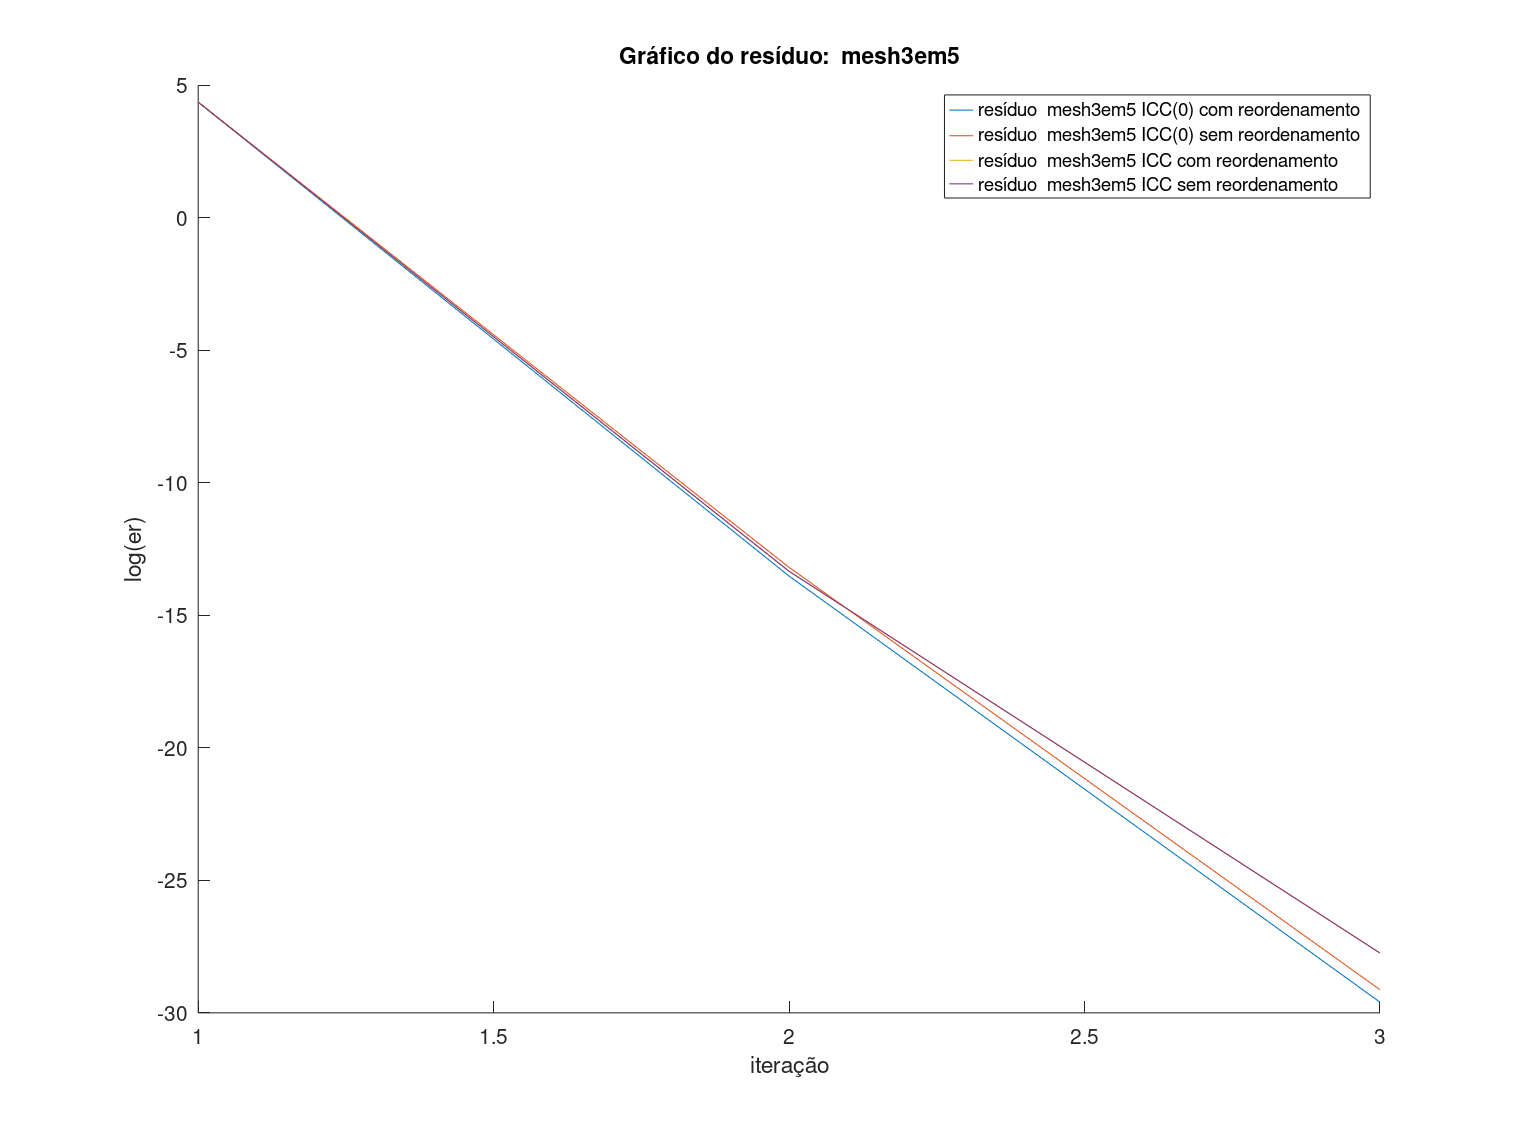
\includegraphics[width=.6\linewidth]{images/mesh3em5.png}
         \caption{Gráfico do Resíduo da matriz \textit{mesh3em5}}
         \label{fig:mesh-res}
\end{figure}

\begin{figure}[H]
    \centering
         \centering
         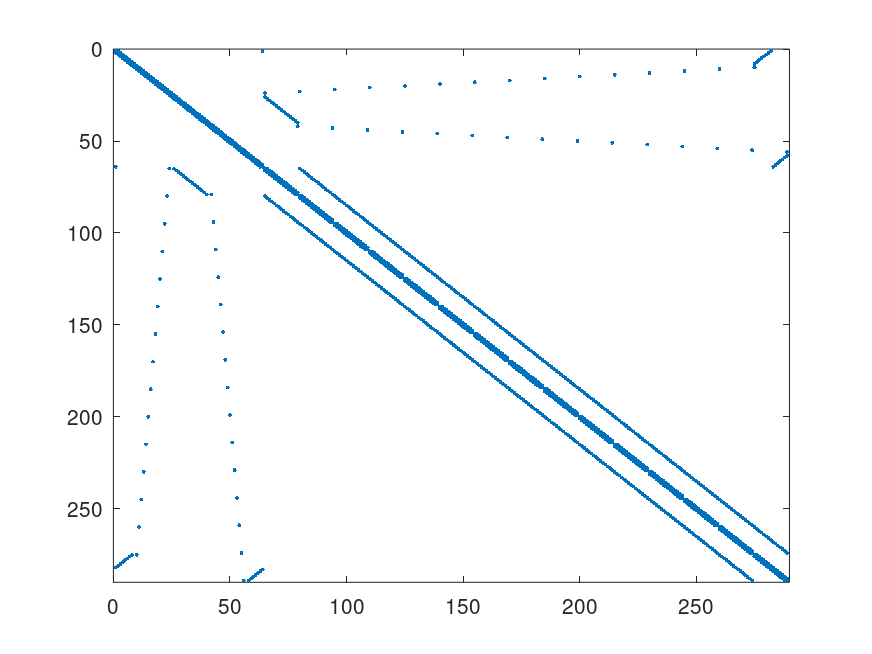
\includegraphics[width=.5\linewidth]{images/mesh3em5_spyA.png}
         \caption{Spy de da matriz \textit{mesh3em5}}
         \label{fig:mesh-spy-a}
\end{figure}

\begin{figure}[H]
    \centering
    \begin{subfigure}[t]{0.4\linewidth}
         \centering
         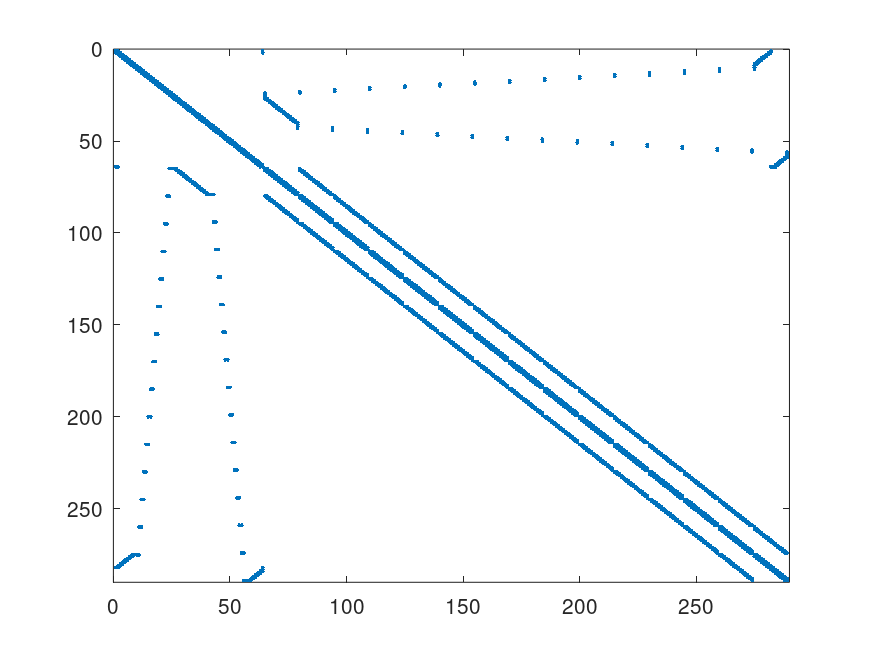
\includegraphics[width=\textwidth]{images/mesh3em5_spyM_ICC(0)_sem.png}
         \caption{Spy após ICC(0) sem reordenamento}
         \label{fig:mesh-icc0-sem}
    \end{subfigure}
    \quad
    \begin{subfigure}[t]{0.4\linewidth}
         \centering
         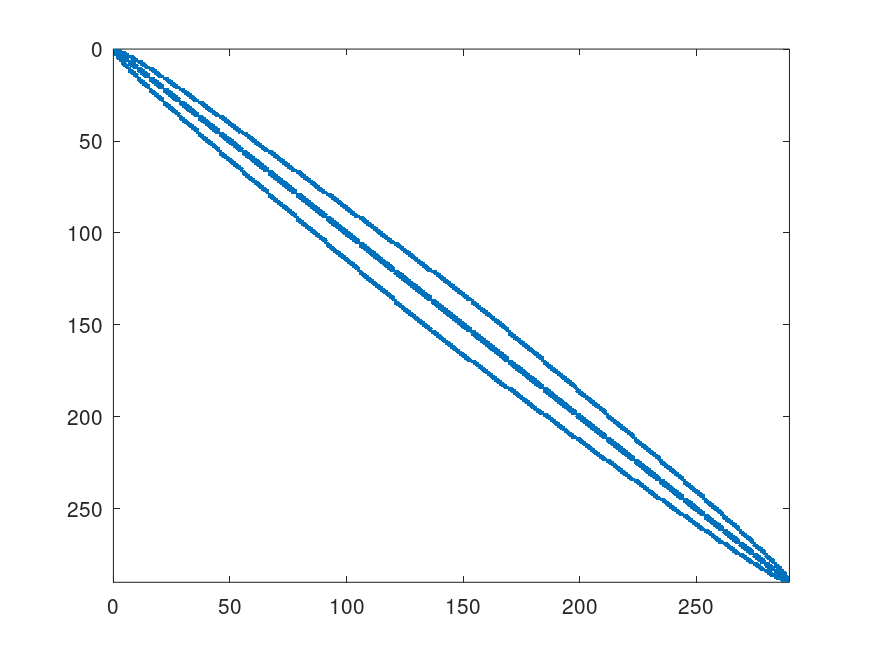
\includegraphics[width=\textwidth]{images/mesh3em5_spyM_ICC(0)_com.png}
         \caption{Spy após ICC(0) com reordenamento}
         \label{fig:mesh-icc0-com}
    \end{subfigure}
    \par\bigskip
    \begin{subfigure}[t]{0.4\linewidth}
         \centering
         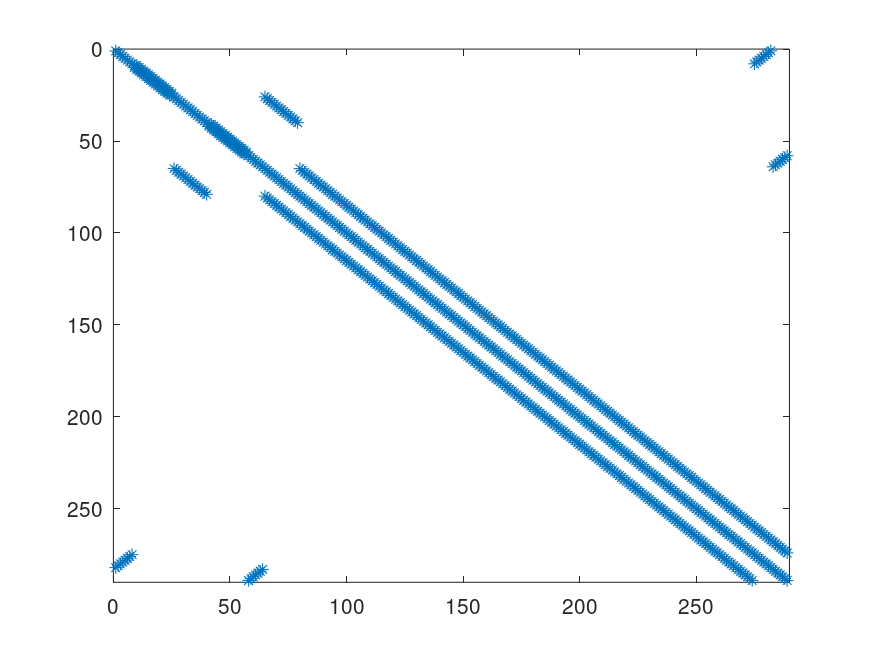
\includegraphics[width=\textwidth]{images/mesh3em5_spyM_ICC_sem.png}
         \caption{Spy após ICC sem reordenamento}
         \label{fig:mesh-icc-s}
    \end{subfigure}
    \quad
    \begin{subfigure}[t]{0.4\linewidth}
         \centering
         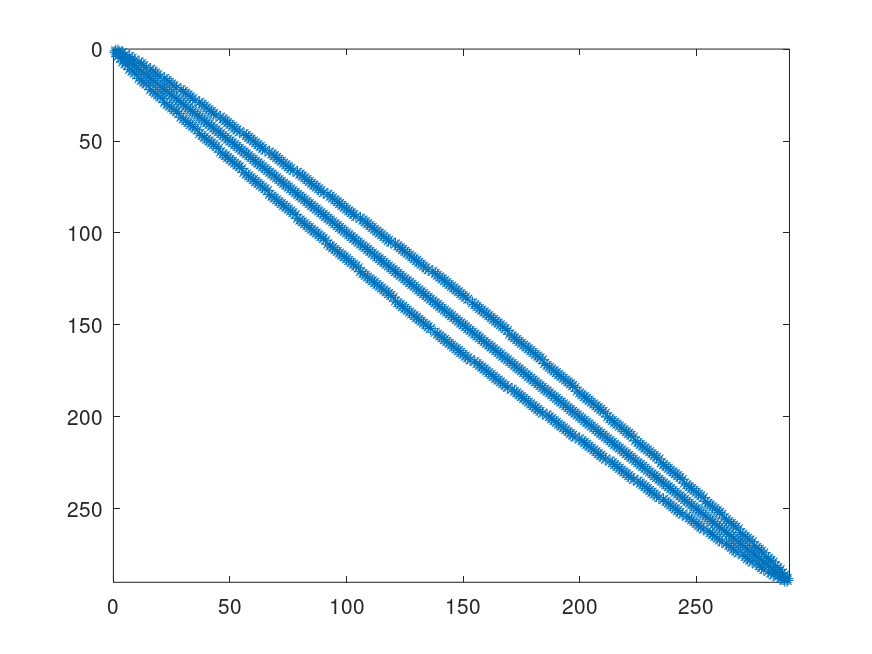
\includegraphics[width=\textwidth]{images/mesh3em5_spyM_ICC_com.png}
         \caption{Spy após ICC com reordenamento}
         \label{fig:mesh-icc-c}
    \end{subfigure}
    \caption{Gráficos do preenchimento de \textit{mesh3em5}.}
    \label{fig:mesh}
\end{figure}
\begin{figure}[H]
    \centering
         \centering
         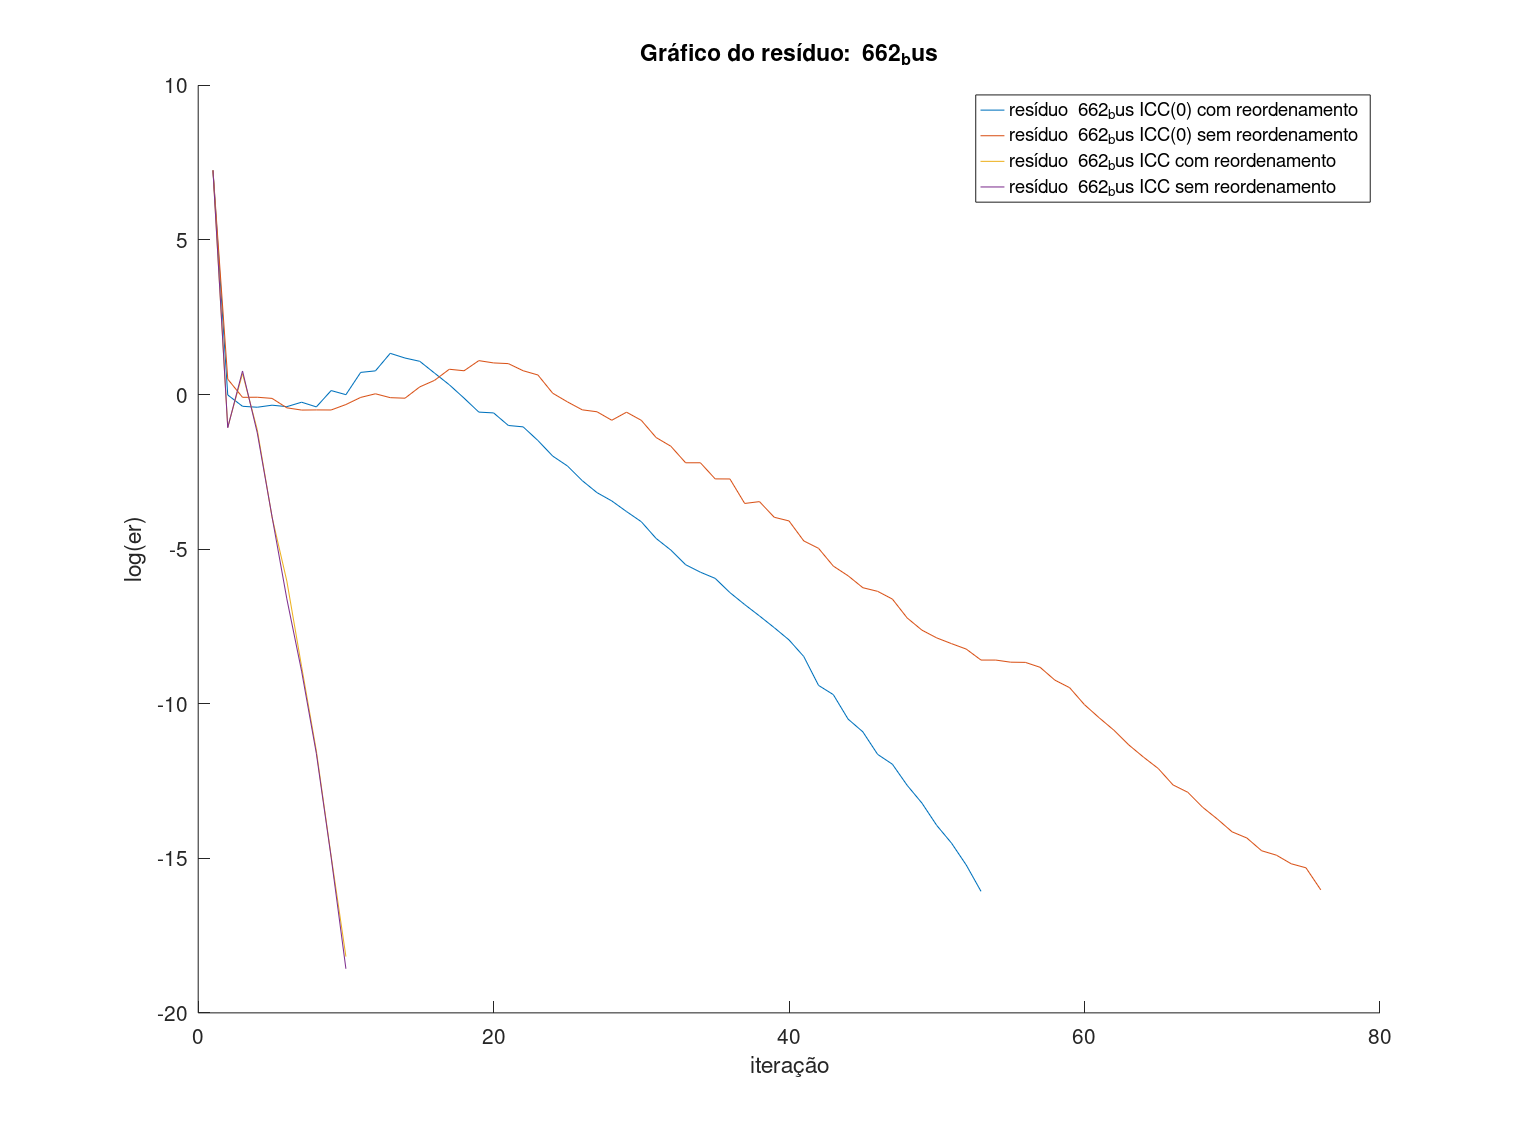
\includegraphics[width=.6\linewidth]{images/662_bus.png}
         \caption{Gráfico do Resíduo da matriz \textit{662\_bus}}
         \label{fig:bus-res}
\end{figure}

\begin{figure}[H]
    \centering
         \centering
         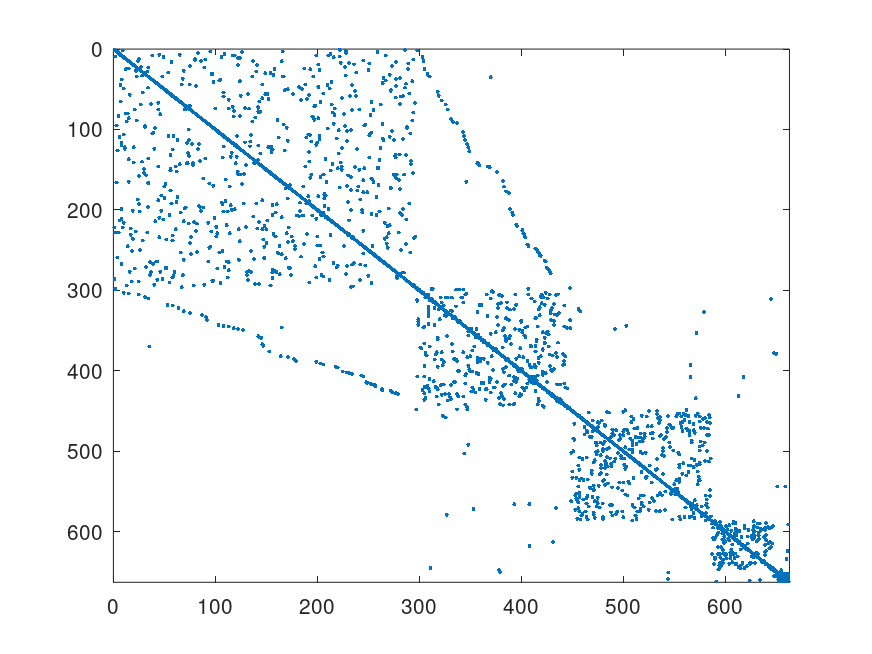
\includegraphics[width=.5\linewidth]{images/662_bus_spyA.png}
         \caption{Spy de da matriz \textit{662\_bus}}
         \label{fig:bus-spy-a}
\end{figure}

\begin{figure}[H]
    \centering
    \begin{subfigure}[t]{0.4\linewidth}
         \centering
         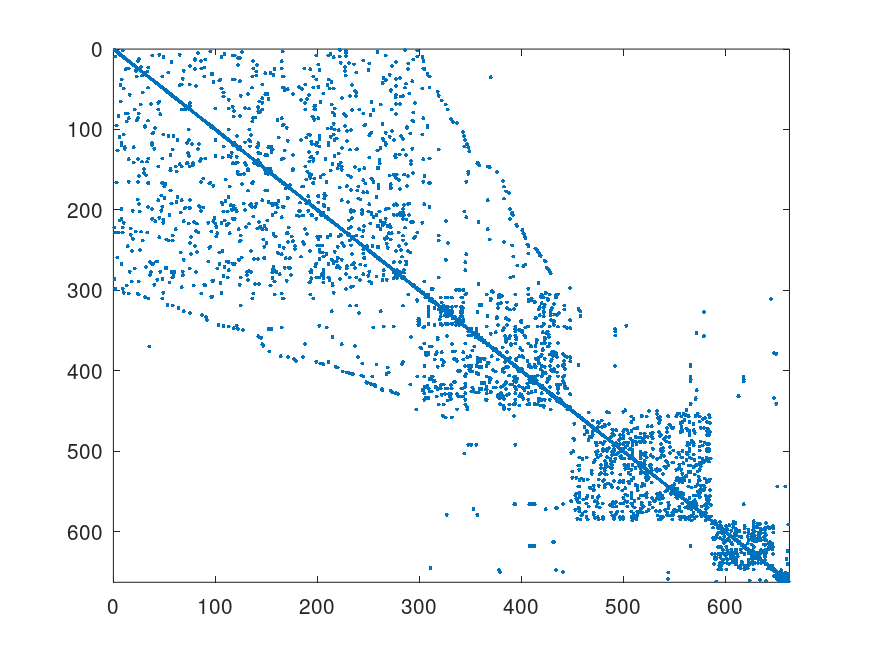
\includegraphics[width=\textwidth]{images/662_bus_spyM_ICC(0)_sem.png}
         \caption{Spy após ICC(0) sem reordenamento}
         \label{fig:bus-icc0-sem}
    \end{subfigure}
    \quad
    \begin{subfigure}[t]{0.4\linewidth}
         \centering
         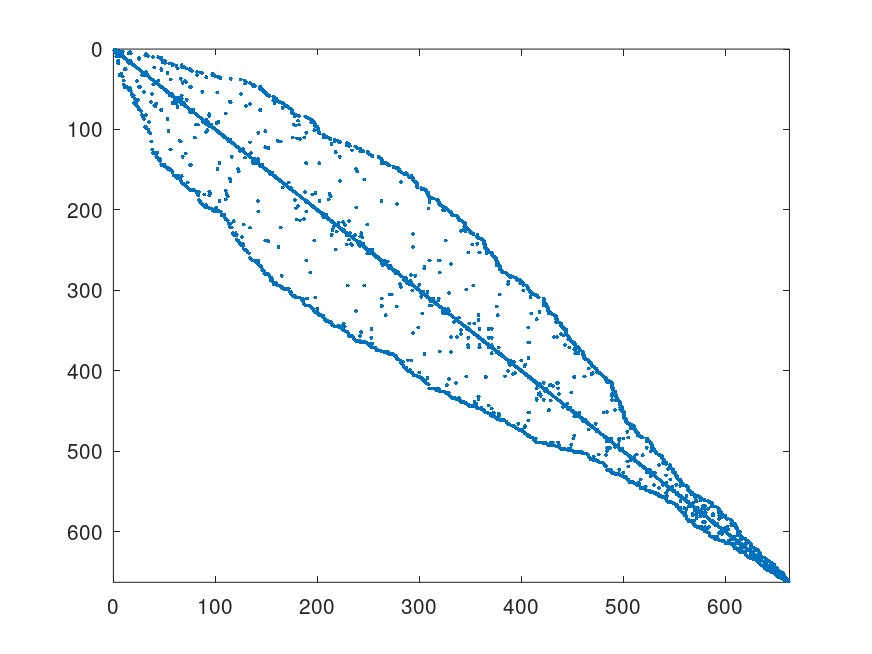
\includegraphics[width=\textwidth]{images/662_bus_spyM_ICC(0)_com.png}
         \caption{Spy após ICC(0) com reordenamento}
         \label{fig:bus-icc0-com}
    \end{subfigure}
    \par\bigskip
    \begin{subfigure}[t]{0.4\linewidth}
         \centering
         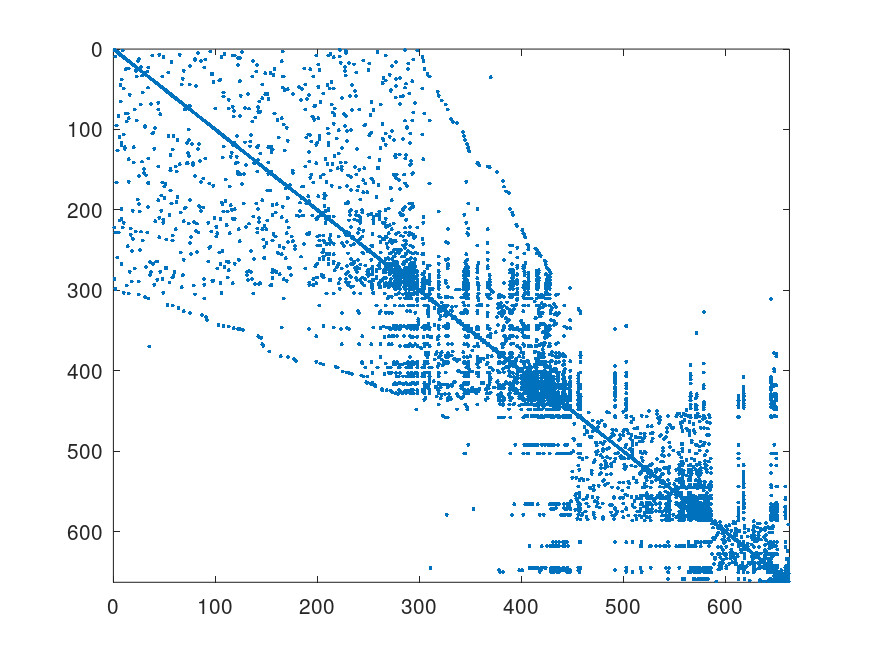
\includegraphics[width=\textwidth]{images/662_bus_spyM_ICC_sem.png}
         \caption{Spy após ICC sem reordenamento}
         \label{fig:bus-icc-s}
    \end{subfigure}
    \quad
    \begin{subfigure}[t]{0.4\linewidth}
         \centering
         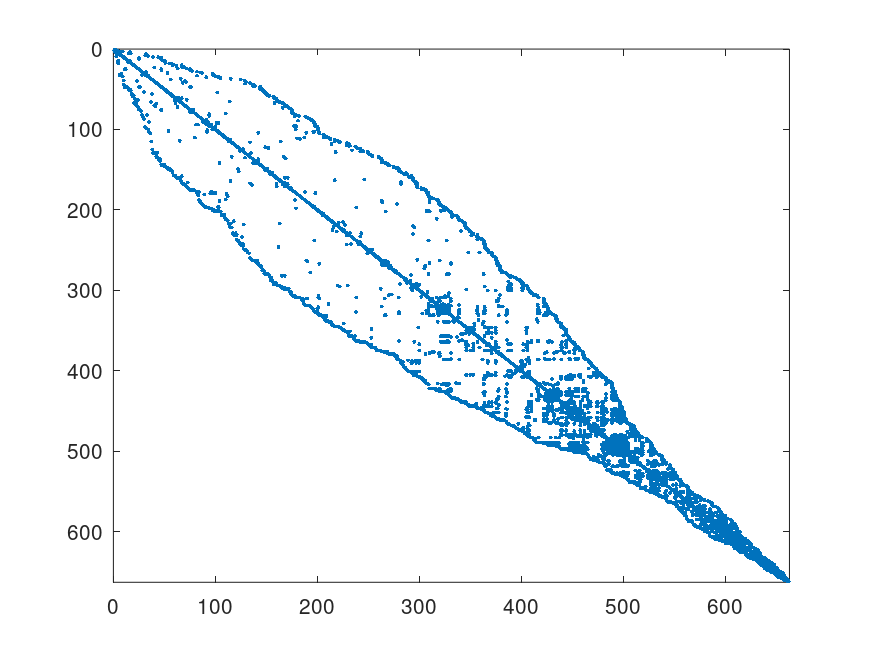
\includegraphics[width=\textwidth]{images/662_bus_spyM_ICC_com.png}
         \caption{Spy após ICC com reordenamento}
         \label{fig:bus-icc-c}
    \end{subfigure}
    \caption{Gráficos do preenchimento de \textit{662\_bus}.}
    \label{fig:bus}
\end{figure}
\begin{figure}[H]
    \centering
         \centering
         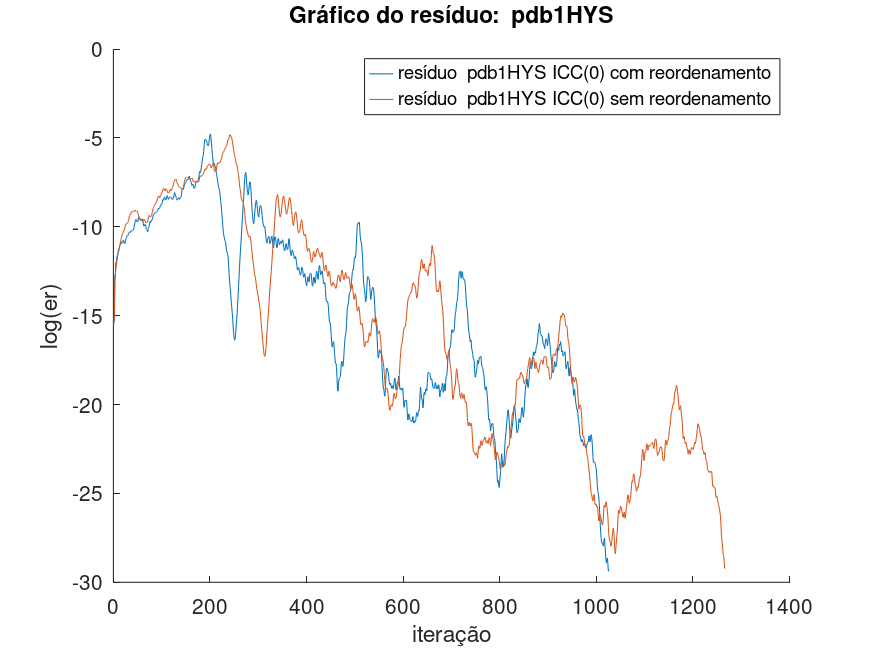
\includegraphics[width=.6\linewidth]{images/pdb1HYS.png}
         \caption{Gráfico do Resíduo da matriz \textit{pdb1HYS}}
         \label{fig:pdb-res}
\end{figure}

\begin{figure}[H]
    \centering
         \centering
         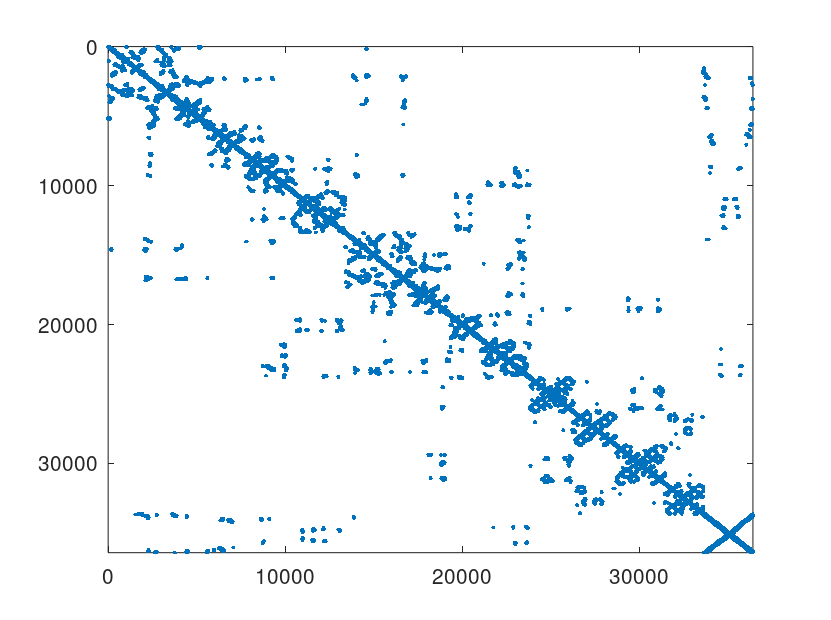
\includegraphics[width=.5\linewidth]{images/pdb1HYS_spyA.png}
         \caption{Spy de da matriz \textit{pdb1HYS}}
         \label{fig:pdb-spy-a}
\end{figure}

\begin{figure}[H]
    \centering
    \begin{subfigure}[t]{0.4\linewidth}
         \centering
         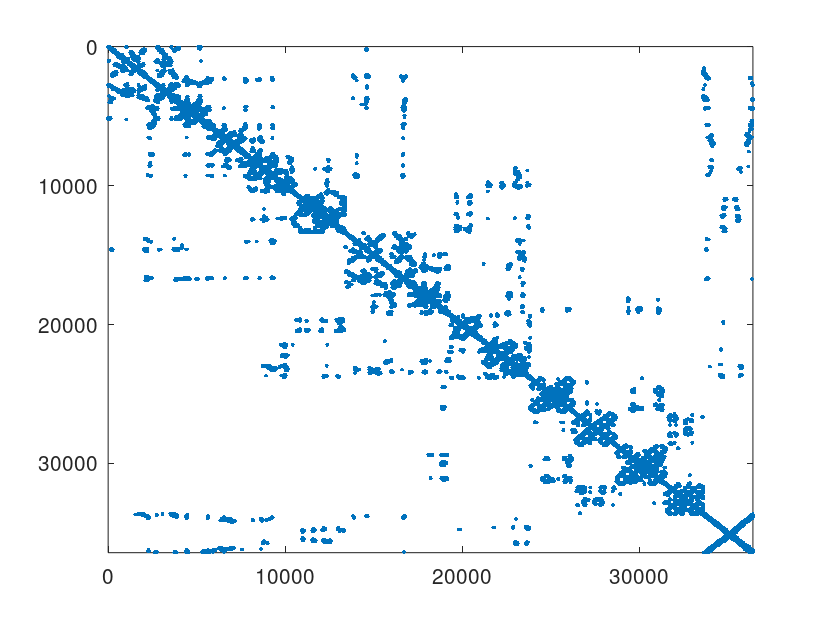
\includegraphics[width=\textwidth]{images/pdb1HYS_spyM_ICC(0)_sem.png}
         \caption{Spy após ICC(0) sem reordenamento}
         \label{fig:pdb-icc0-sem}
    \end{subfigure}
    \quad
    \begin{subfigure}[t]{0.4\linewidth}
         \centering
         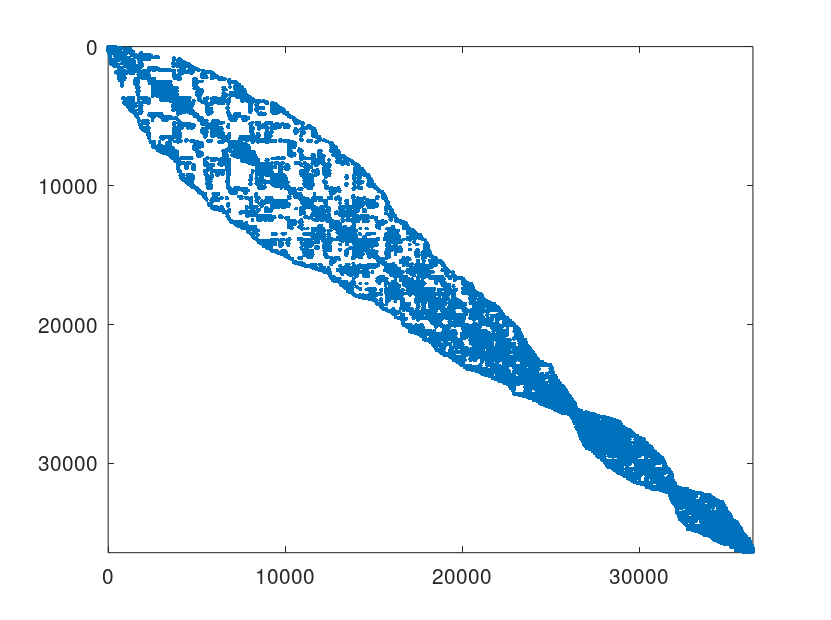
\includegraphics[width=\textwidth]{images/pdb1HYS_spyM_ICC(0)_com.png}
         \caption{Spy após ICC(0) com reordenamento}
         \label{fig:pdb-icc0-com}
    \end{subfigure}
    \label{fig:pdb}
\end{figure}
\begin{figure}[H]
    \centering
         \centering
         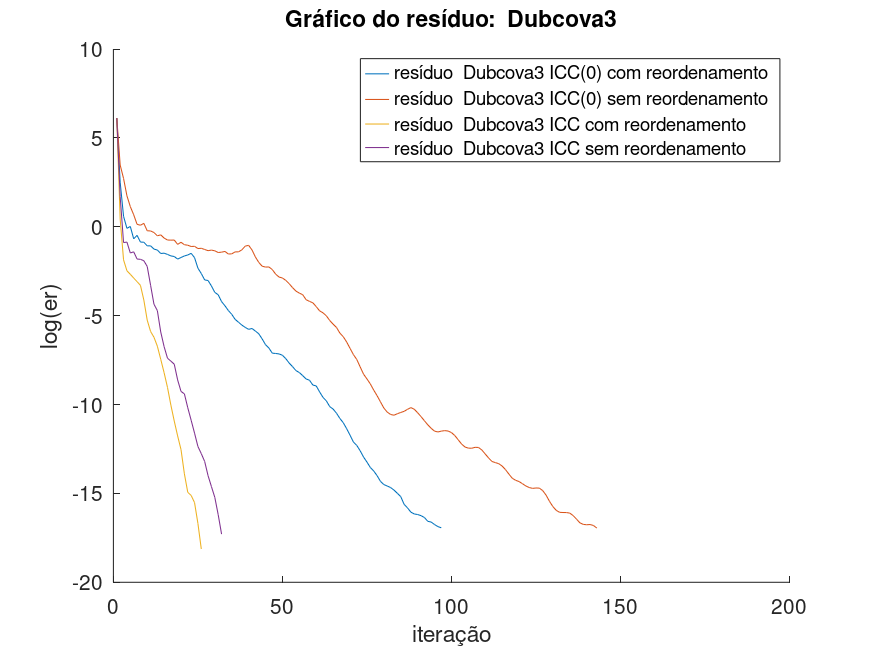
\includegraphics[width=.6\linewidth]{images/Dubcova3.png}
         \caption{Gráfico do Resíduo da matriz \textit{Dubcova3}}
         \label{fig:Dub-res}
\end{figure}


\begin{figure}[H]
    \centering
         \centering
         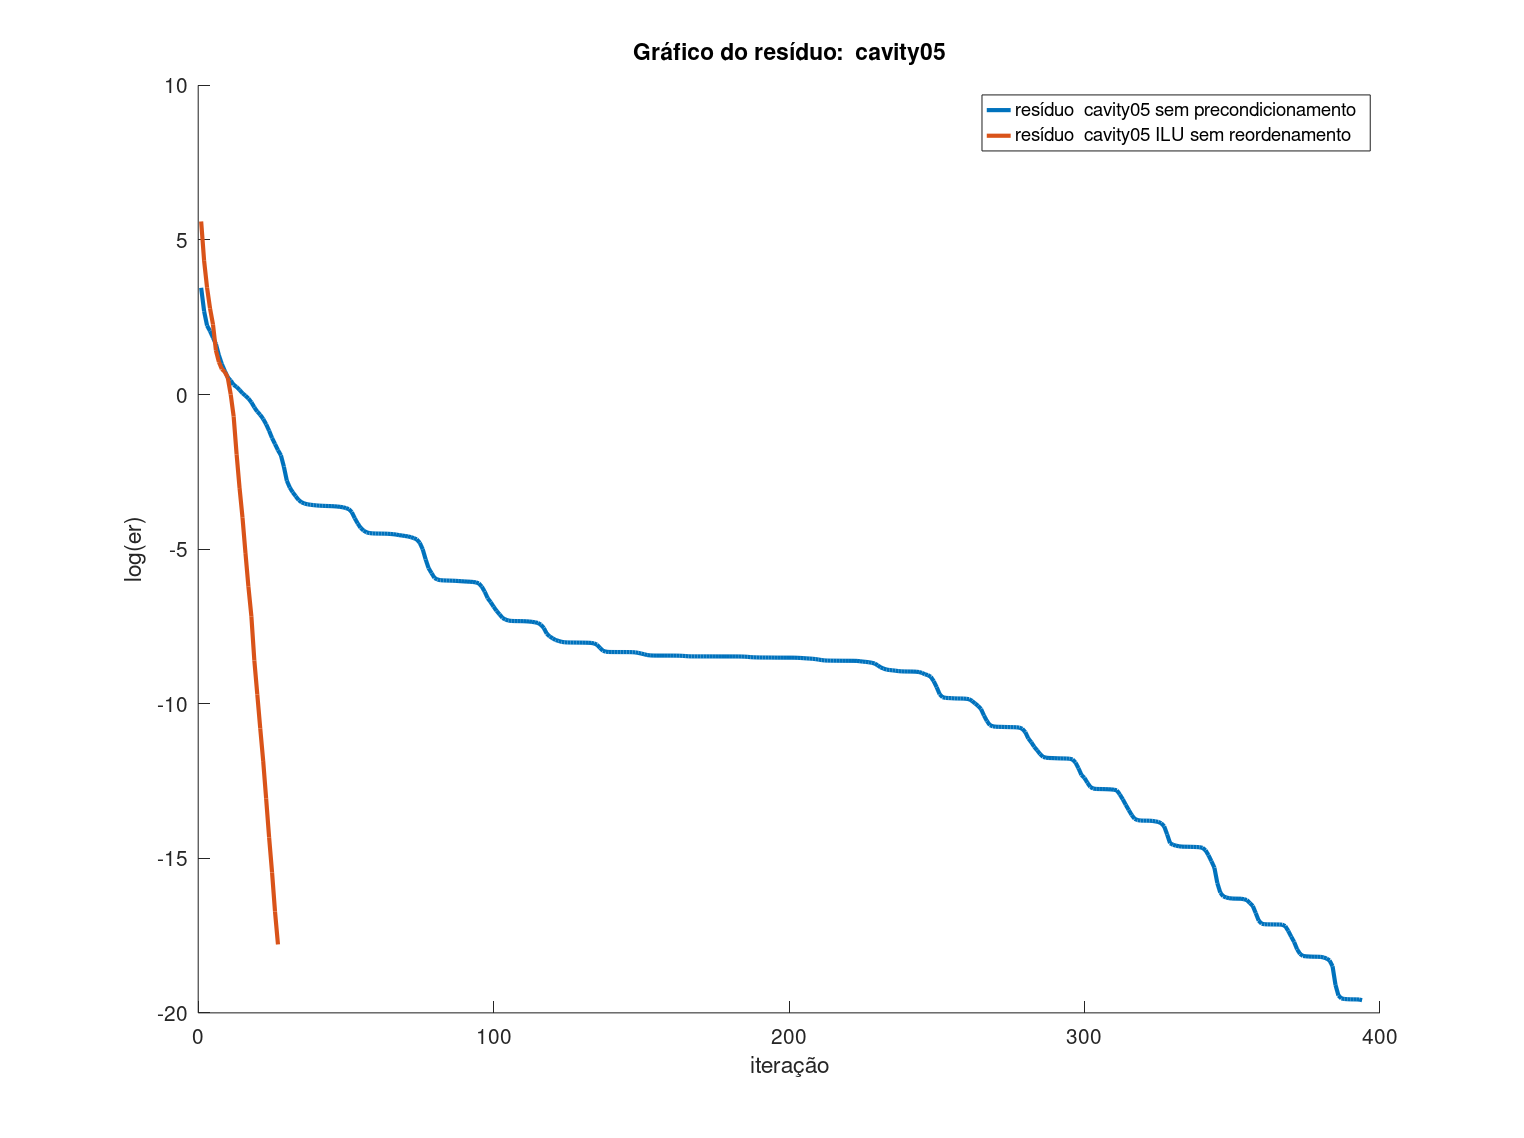
\includegraphics[width=.6\linewidth]{images/cavity05.png}
         \caption{Gráfico do Resíduo da matriz \textit{cavity05}}
         \label{fig:cavity-res}
\end{figure}

\begin{figure}[H]
    \centering
         \centering
         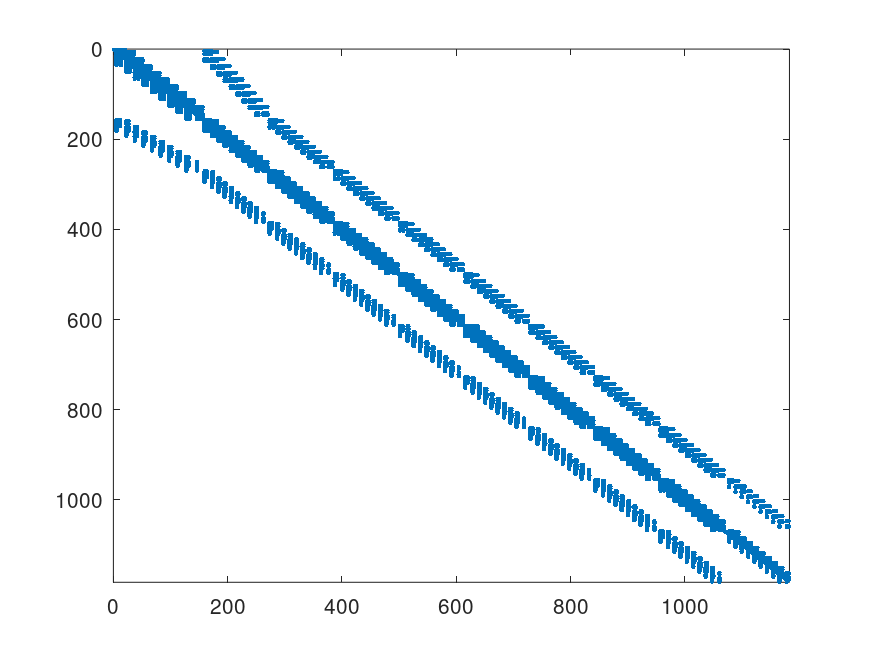
\includegraphics[width=.5\linewidth]{images/cavity05_spyA.png}
         \caption{Spy de da matriz \textit{cavity05}}
         \label{fig:cavity-spy-a}
\end{figure}

\begin{figure}[H]
    \centering
    \begin{subfigure}[t]{0.4\linewidth}
         \centering
         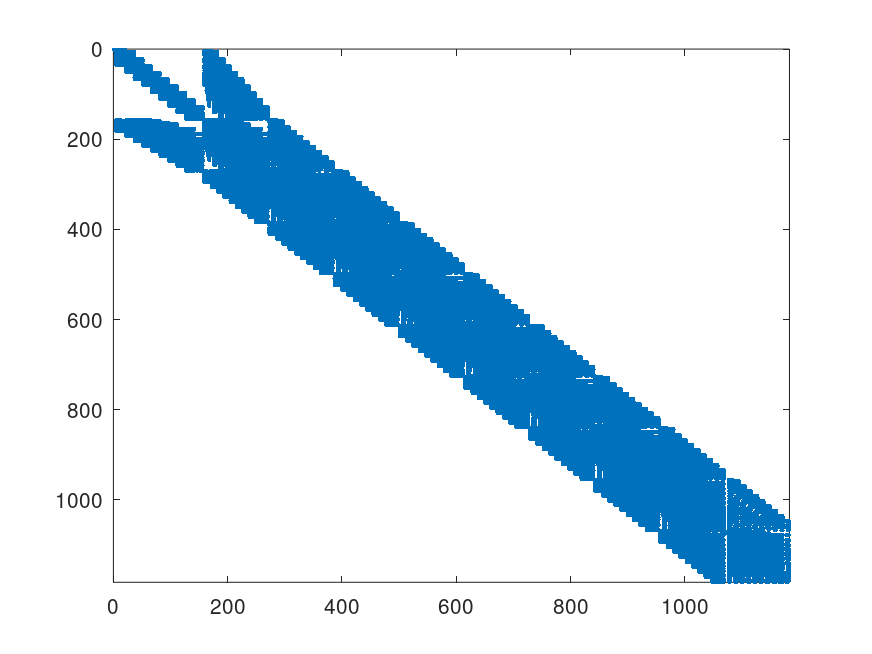
\includegraphics[width=\textwidth]{images/cavity05_spyM_ILU_sem.png}
         \caption{Spy após ILU sem reordenamento}
         \label{fig:cavity-ILU-s}
    \end{subfigure}
    \quad
    \begin{subfigure}[t]{0.4\linewidth}
         \centering
         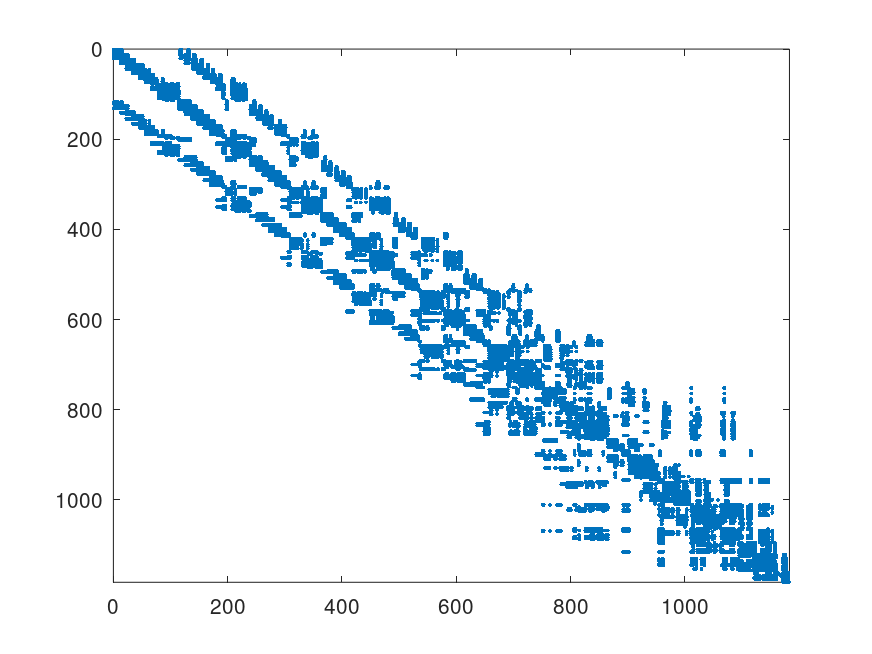
\includegraphics[width=\textwidth]{images/cavity05_spyM_ILU_com.png}
         \caption{Spy após ILU com reordenamento}
         \label{fig:cavity-ILU-c}
    \end{subfigure}
    \caption{Gráficos do preenchimento de \textit{cavity05}.}
    \label{fig:cavity}
\end{figure}
\begin{figure}[H]
    \centering
         \centering
         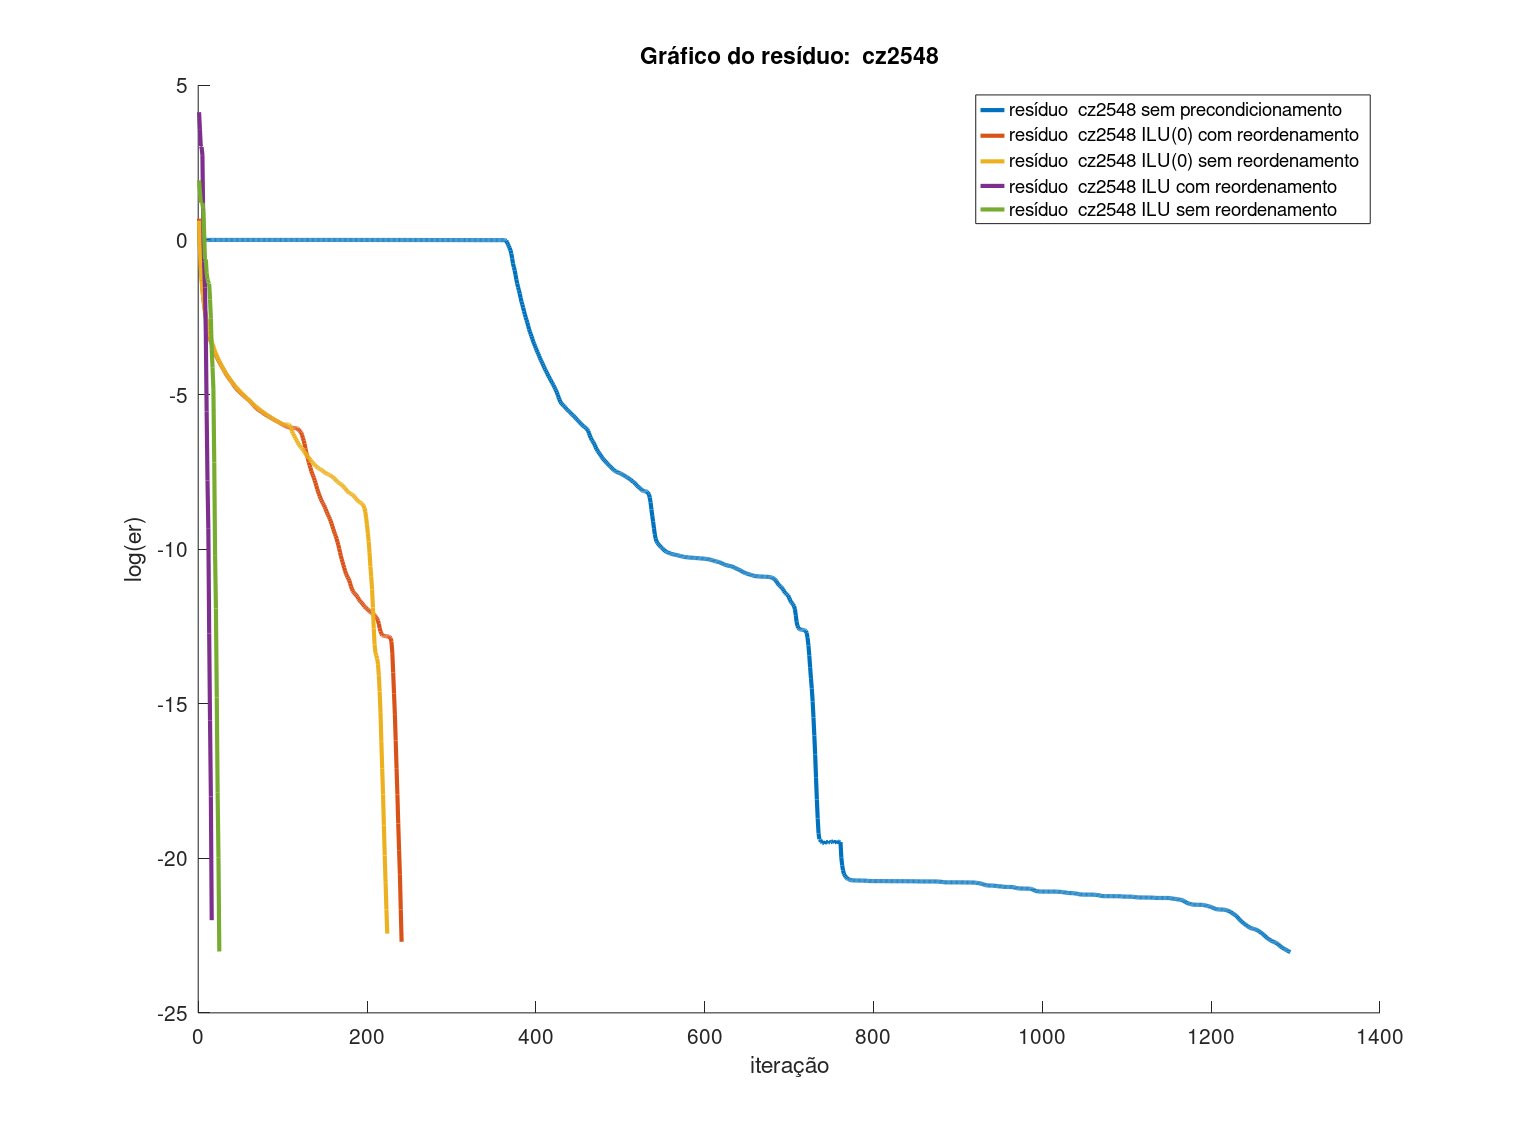
\includegraphics[width=.6\linewidth]{images/cz2548.png}
         \caption{Gráfico do Resíduo da matriz \textit{cz2548}}
         \label{fig:cz-res}
\end{figure}

\begin{figure}[H]
    \centering
         \centering
         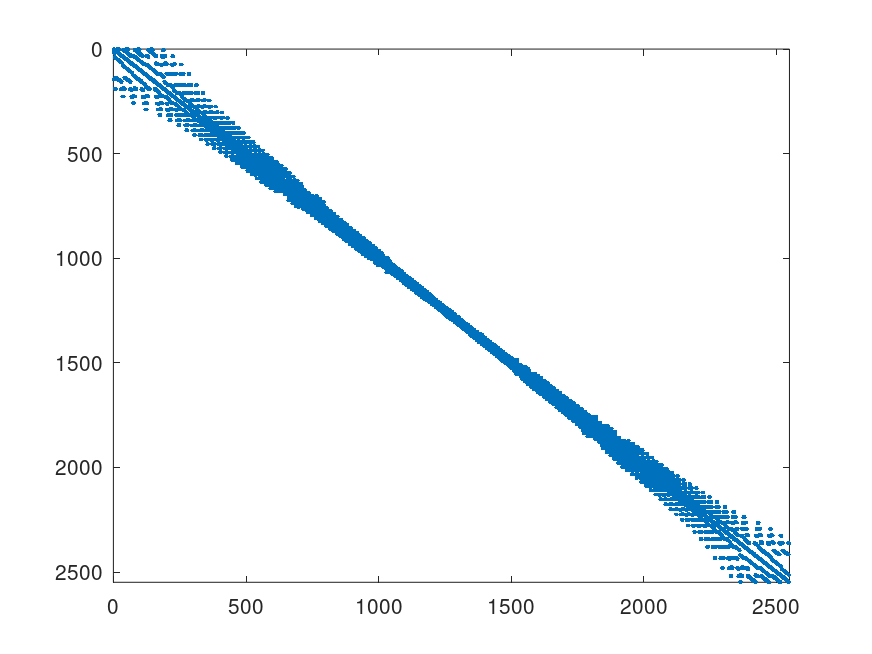
\includegraphics[width=.5\linewidth]{images/cz2548_spyA.png}
         \caption{Spy de da matriz \textit{cz2548}}
         \label{fig:cz-spy-a}
\end{figure}

\begin{figure}[H]
    \centering
    \begin{subfigure}[t]{0.4\linewidth}
         \centering
         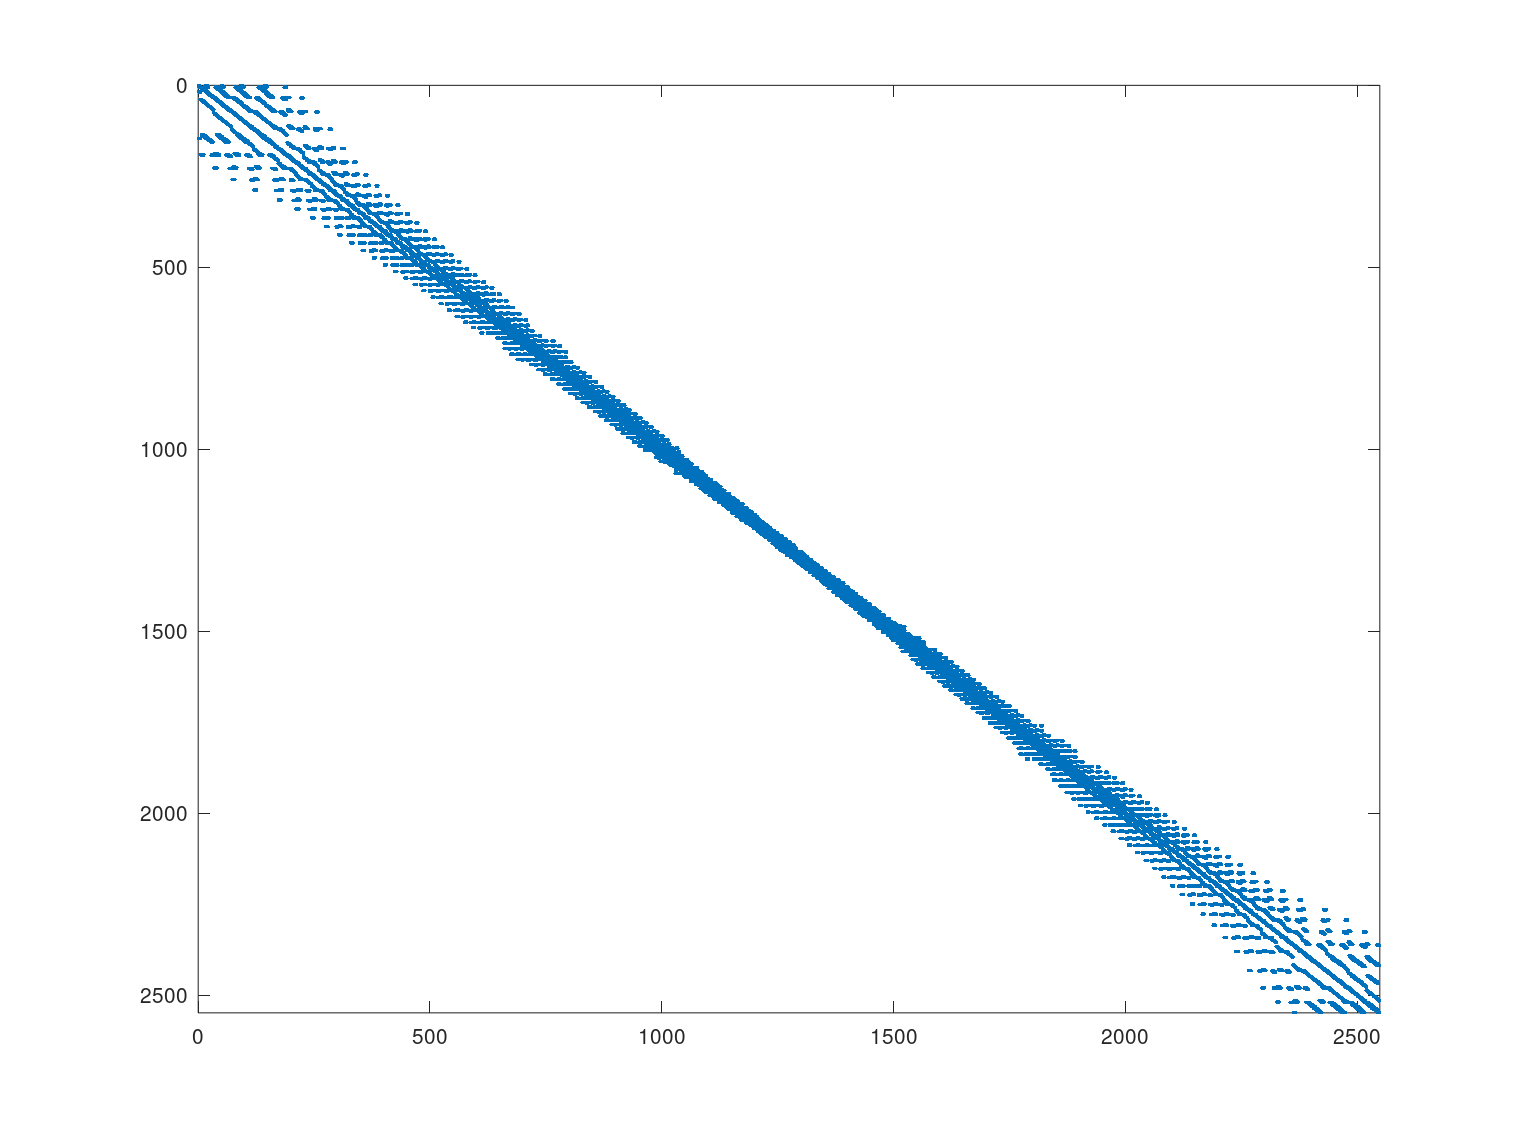
\includegraphics[width=\textwidth]{images/cz2548_spyM_ILU(0)_sem.png}
         \caption{Spy após ILU(0) sem reordenamento}
         \label{fig:cz-ILU0-sem}
    \end{subfigure}
    \quad
    \begin{subfigure}[t]{0.4\linewidth}
         \centering
         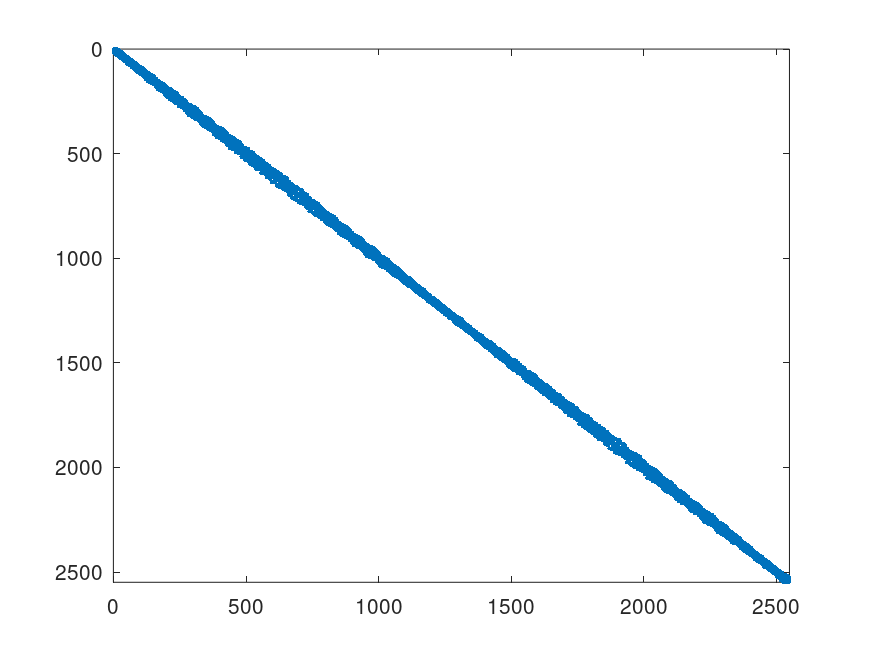
\includegraphics[width=\textwidth]{images/cz2548_spyM_ILU(0)_com.png}
         \caption{Spy após ILU(0) com reordenamento}
         \label{fig:cz-ILU0-com}
    \end{subfigure}
    \par\bigskip
    \begin{subfigure}[t]{0.4\linewidth}
         \centering
         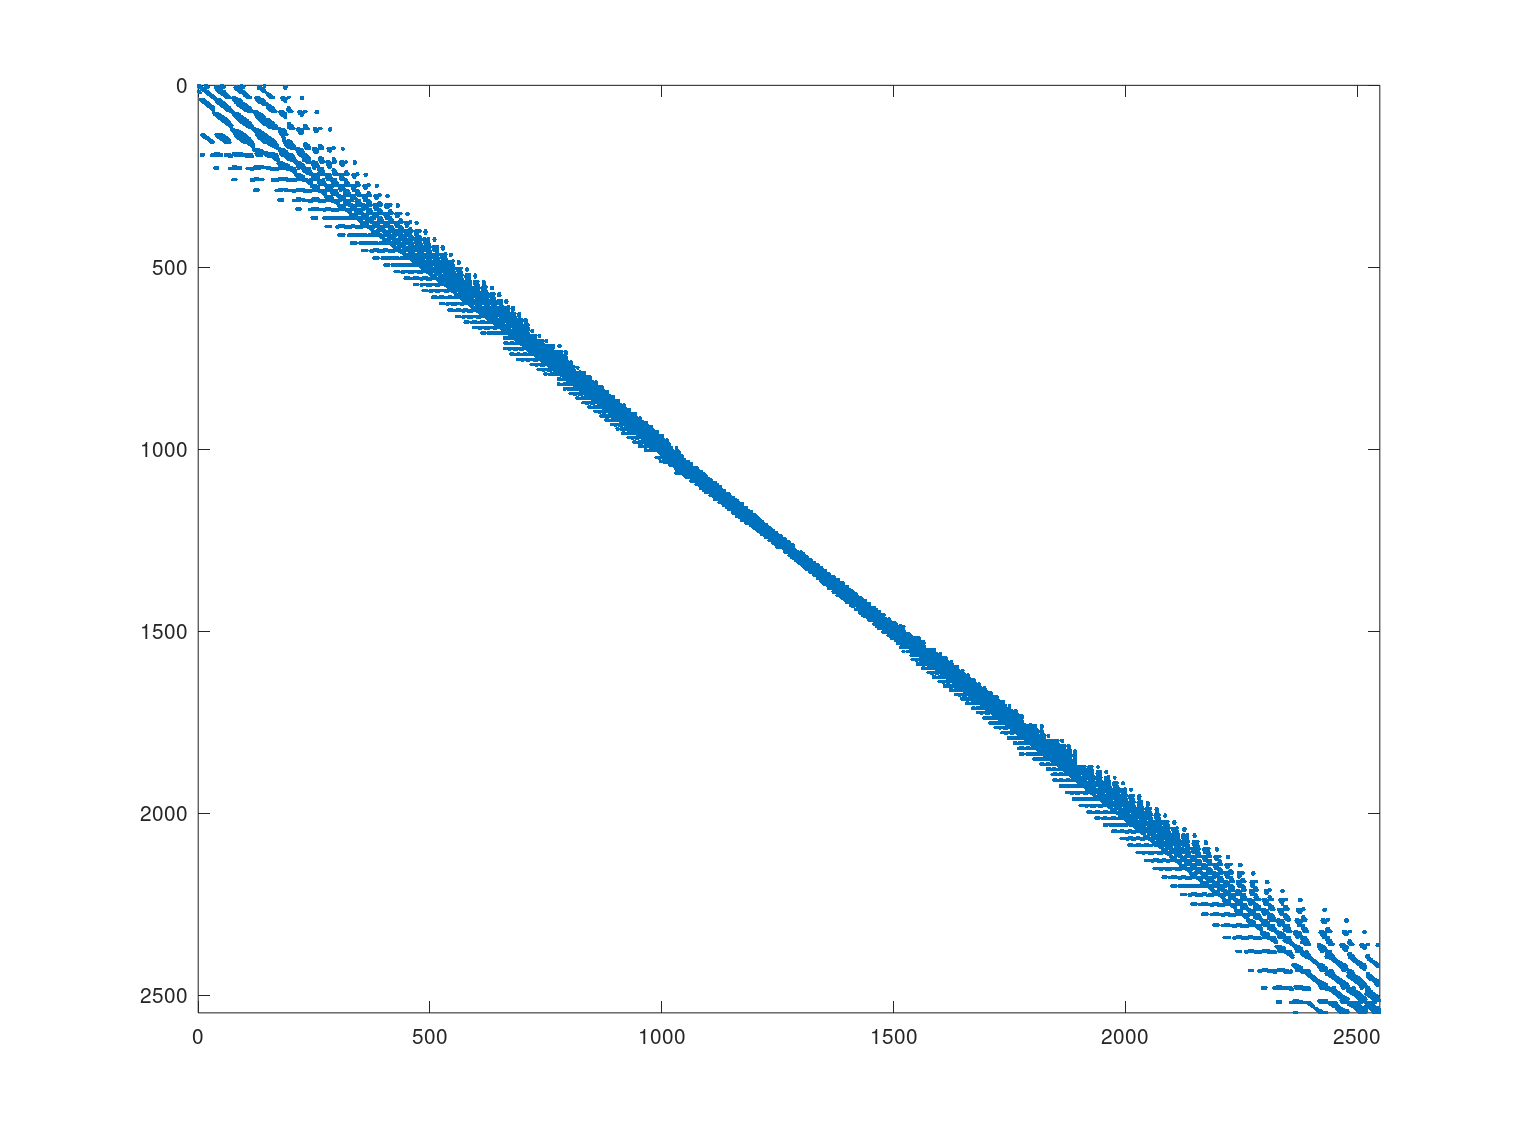
\includegraphics[width=\textwidth]{images/cz2548_spyM_ILU_sem.png}
         \caption{Spy após ILU sem reordenamento}
         \label{fig:cz-ILU-s}
    \end{subfigure}
    \quad
    \begin{subfigure}[t]{0.4\linewidth}
         \centering
         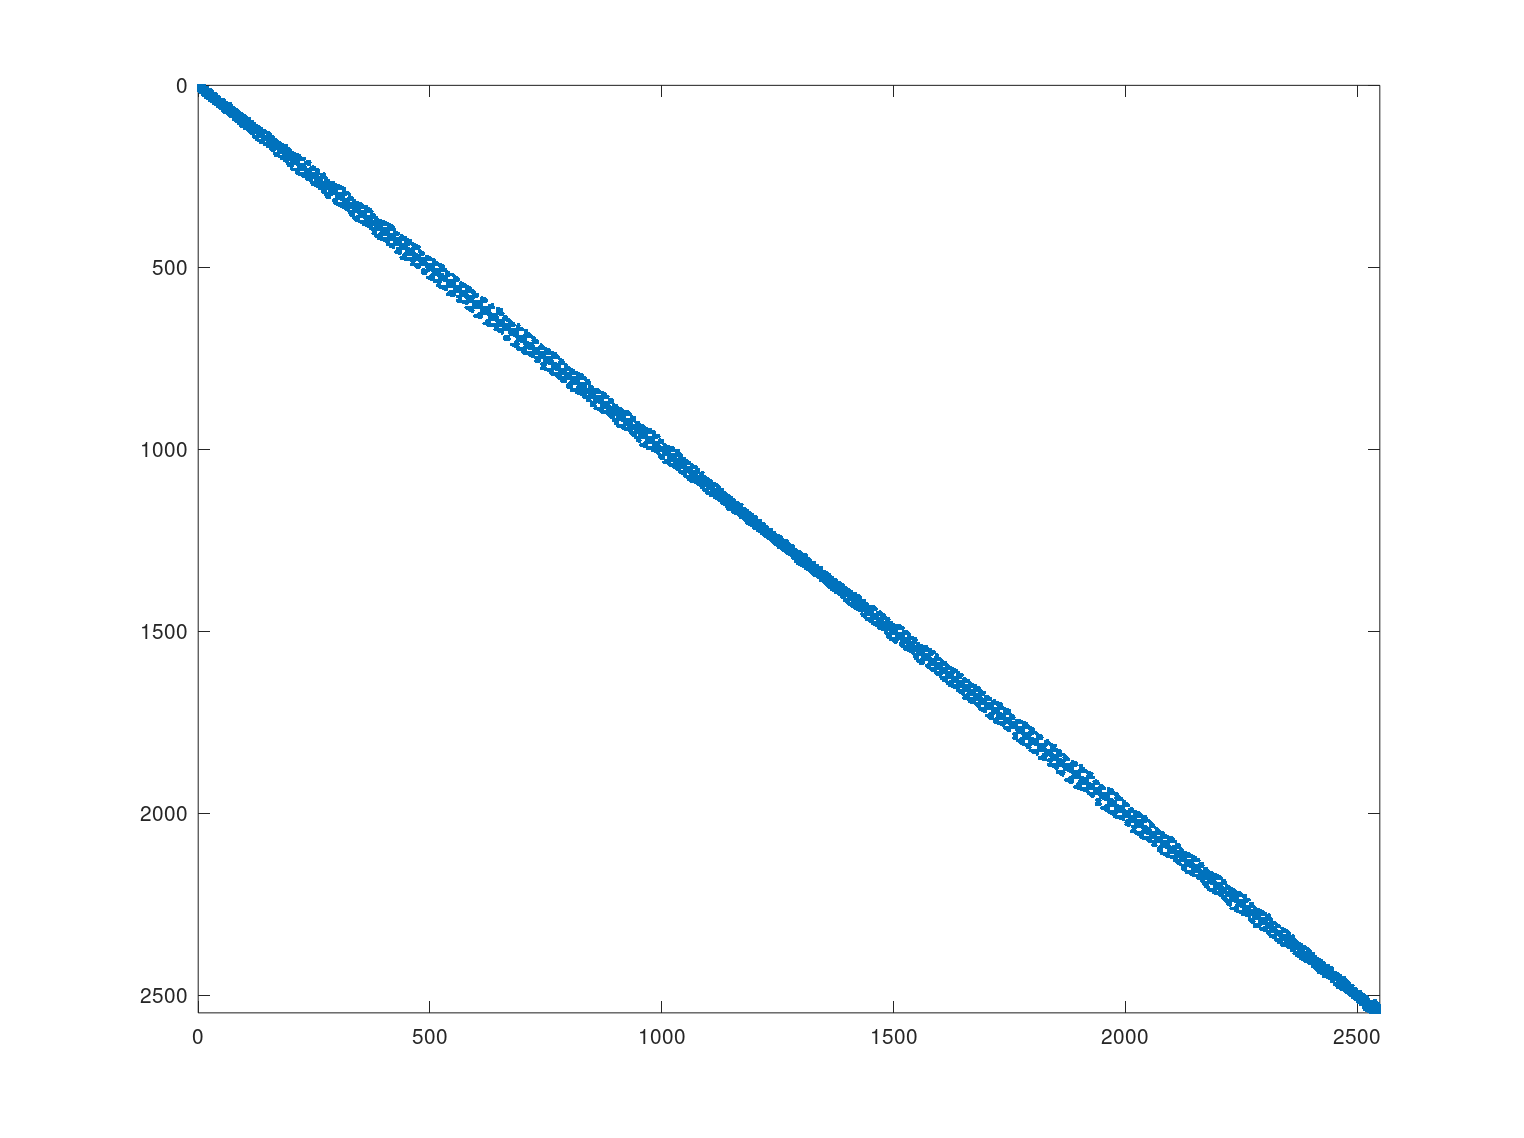
\includegraphics[width=\textwidth]{images/cz2548_spyM_ILU_com.png}
         \caption{Spy após ILU com reordenamento}
         \label{fig:cz-ILU-c}
    \end{subfigure}
    \caption{Gráficos do preenchimento de \textit{cz2548}.}
    \label{fig:cz}
\end{figure}
\begin{figure}[H]
    \centering
         \centering
         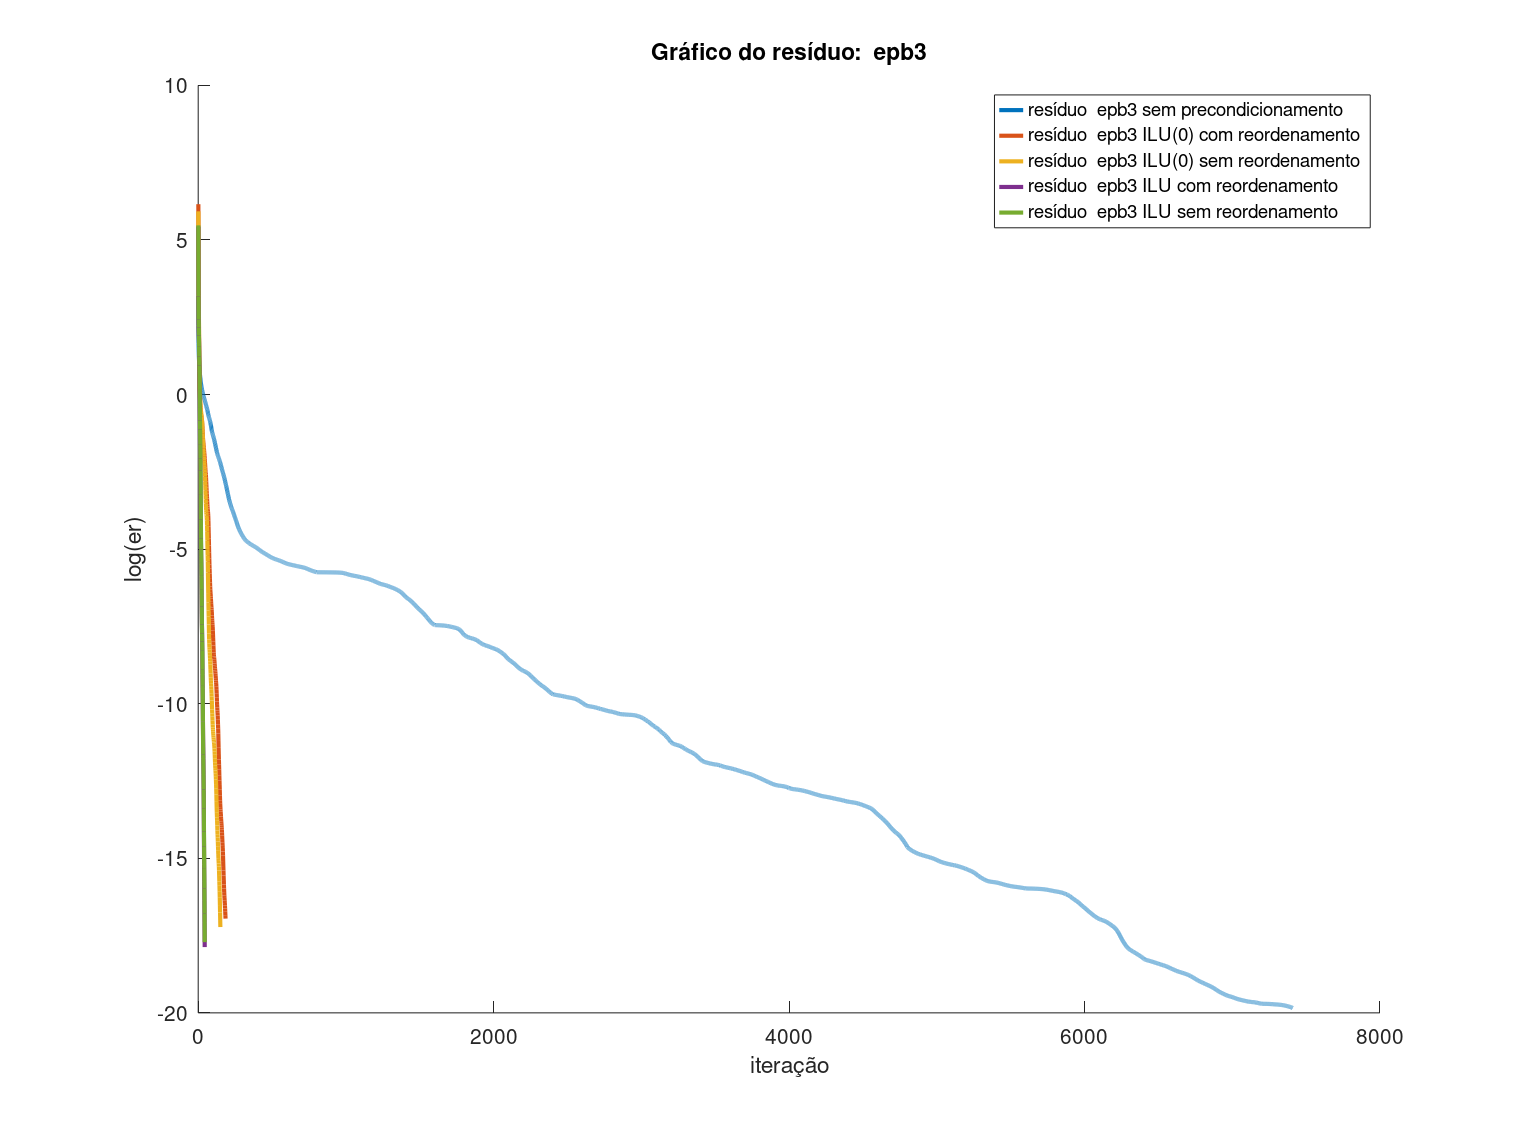
\includegraphics[width=.6\linewidth]{images/epb3.png}
         \caption{Gráfico do Resíduo da matriz \textit{epb3}}
         \label{fig:epb-res}
\end{figure}

\begin{figure}[H]
    \centering
         \centering
         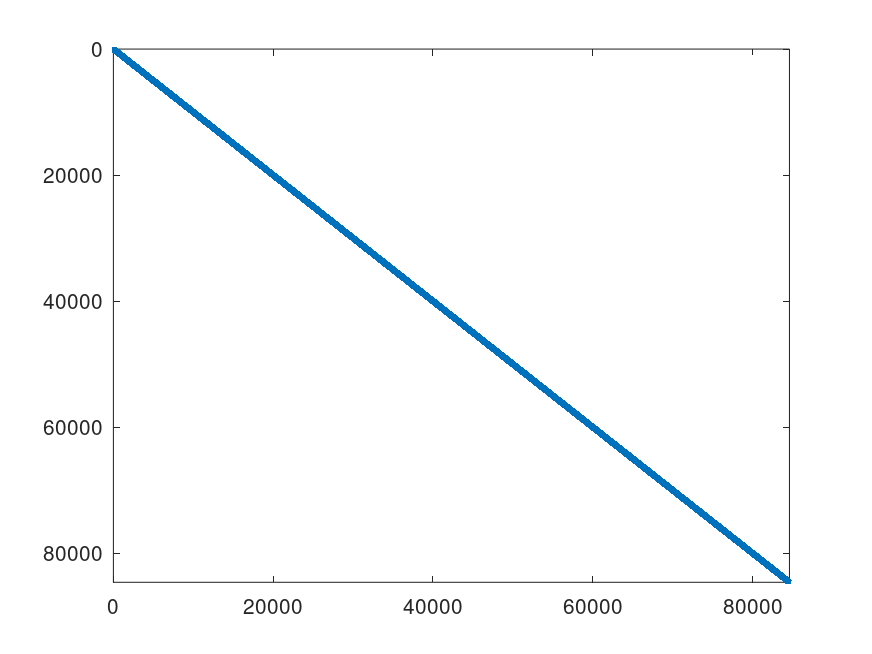
\includegraphics[width=.5\linewidth]{images/epb3_spyA.png}
         \caption{Spy de da matriz \textit{epb3}}
         \label{fig:epb-spy-a}
\end{figure}

\begin{figure}[H]
    \centering
    \begin{subfigure}[t]{0.4\linewidth}
         \centering
         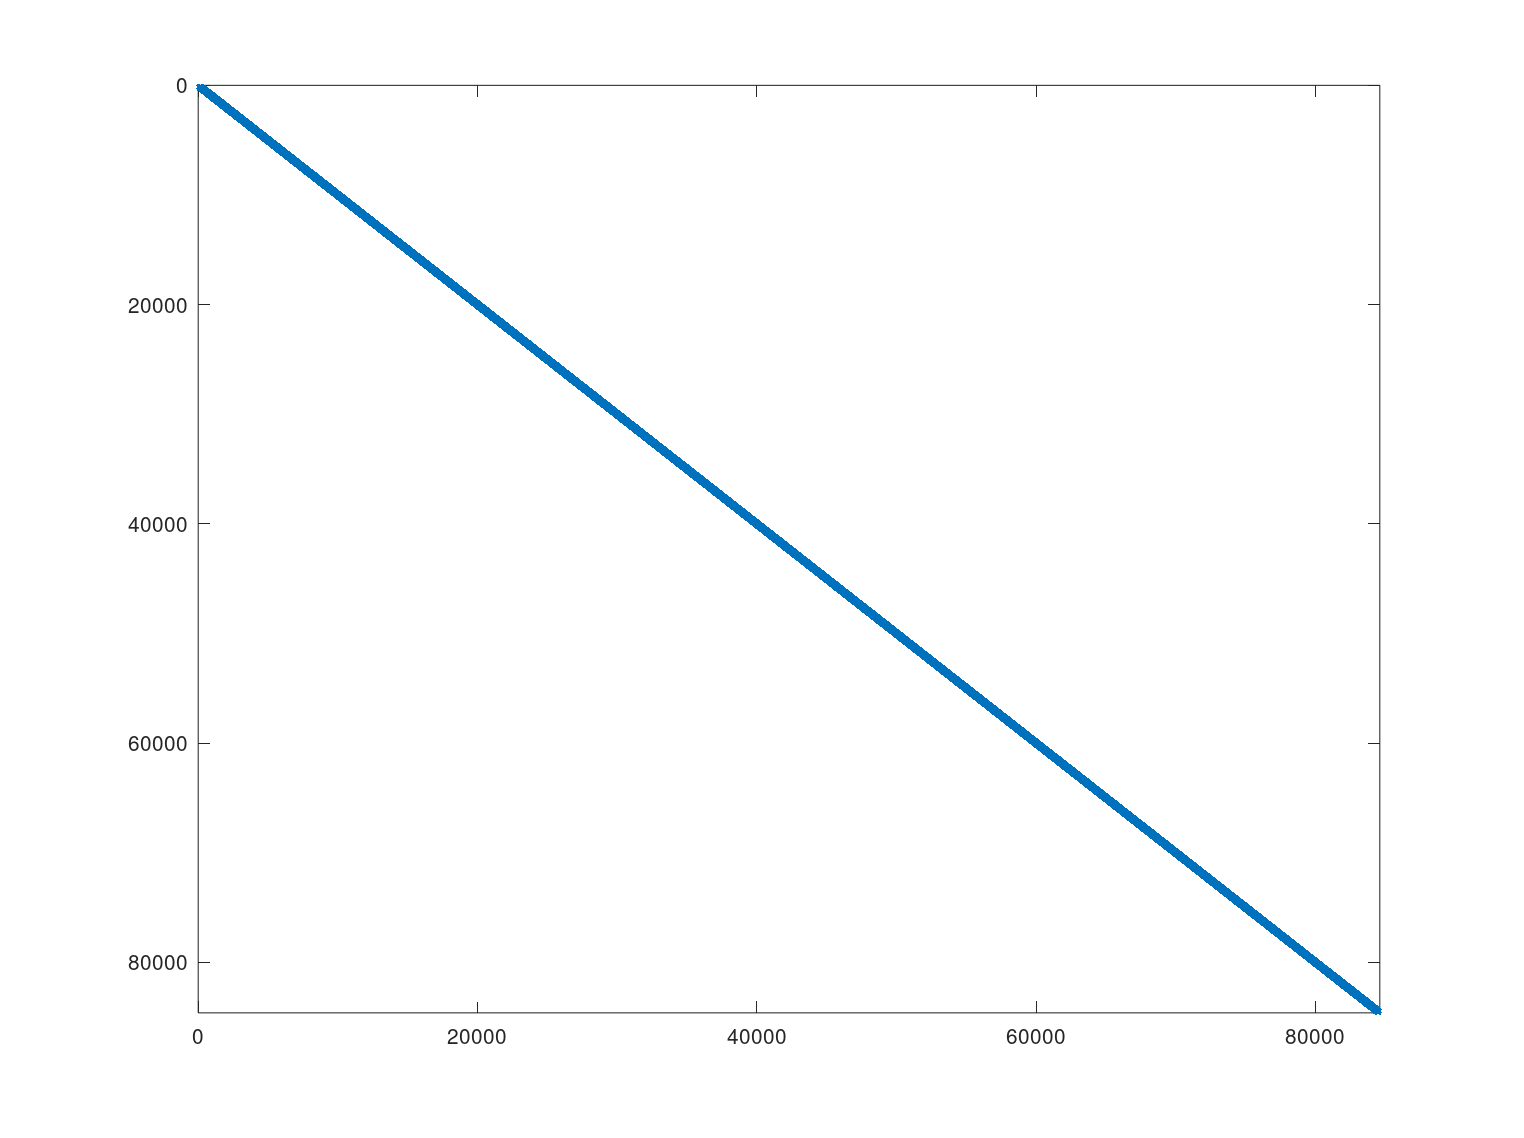
\includegraphics[width=\textwidth]{images/epb3_spyM_ILU(0)_sem.png}
         \caption{Spy após ILU(0) sem reordenamento}
         \label{fig:epb-ILU0-sem}
    \end{subfigure}
    \quad
    \begin{subfigure}[t]{0.4\linewidth}
         \centering
         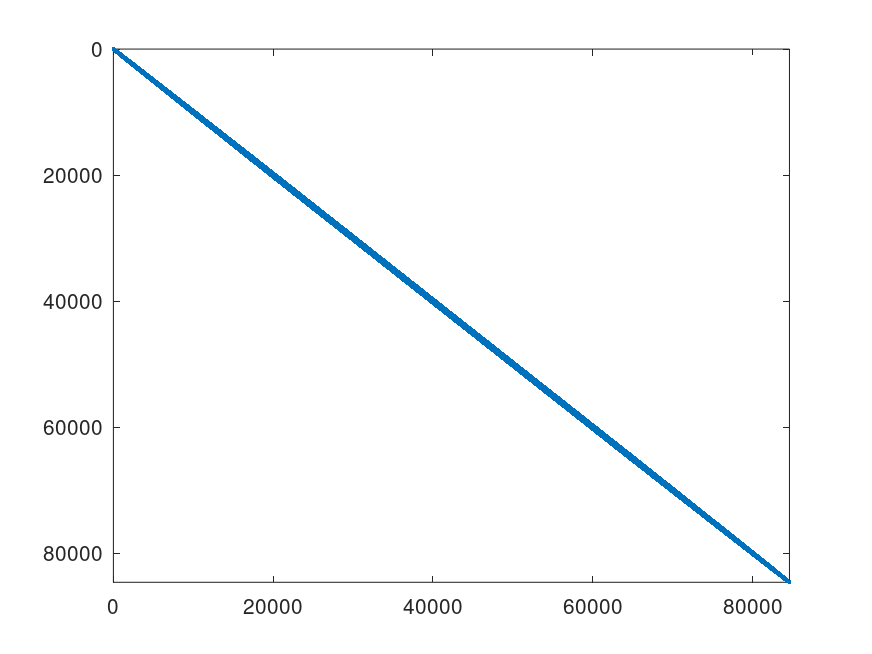
\includegraphics[width=\textwidth]{images/epb3_spyM_ILU(0)_com.png}
         \caption{Spy após ILU(0) com reordenamento}
         \label{fig:epb-ILU0-com}
    \end{subfigure}
    \par\bigskip
    \begin{subfigure}[t]{0.4\linewidth}
         \centering
         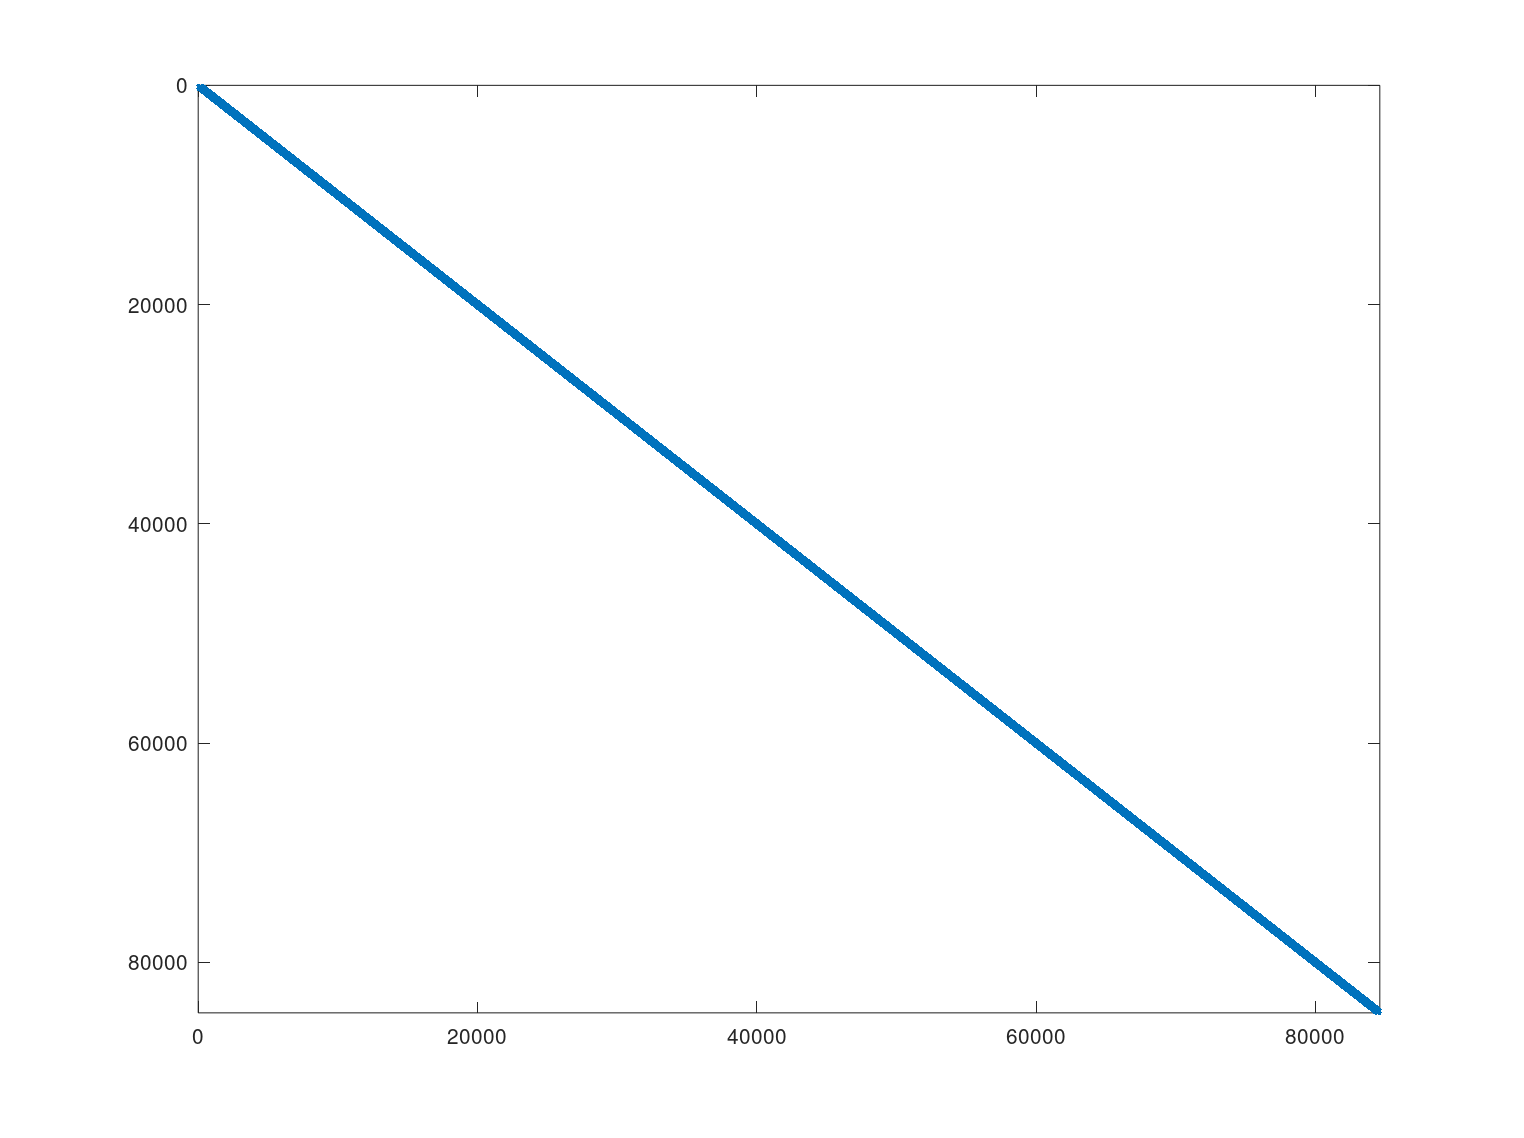
\includegraphics[width=\textwidth]{images/epb3_spyM_ILU_sem.png}
         \caption{Spy após ILU sem reordenamento}
         \label{fig:epb-ILU-s}
    \end{subfigure}
    \quad
    \begin{subfigure}[t]{0.4\linewidth}
         \centering
         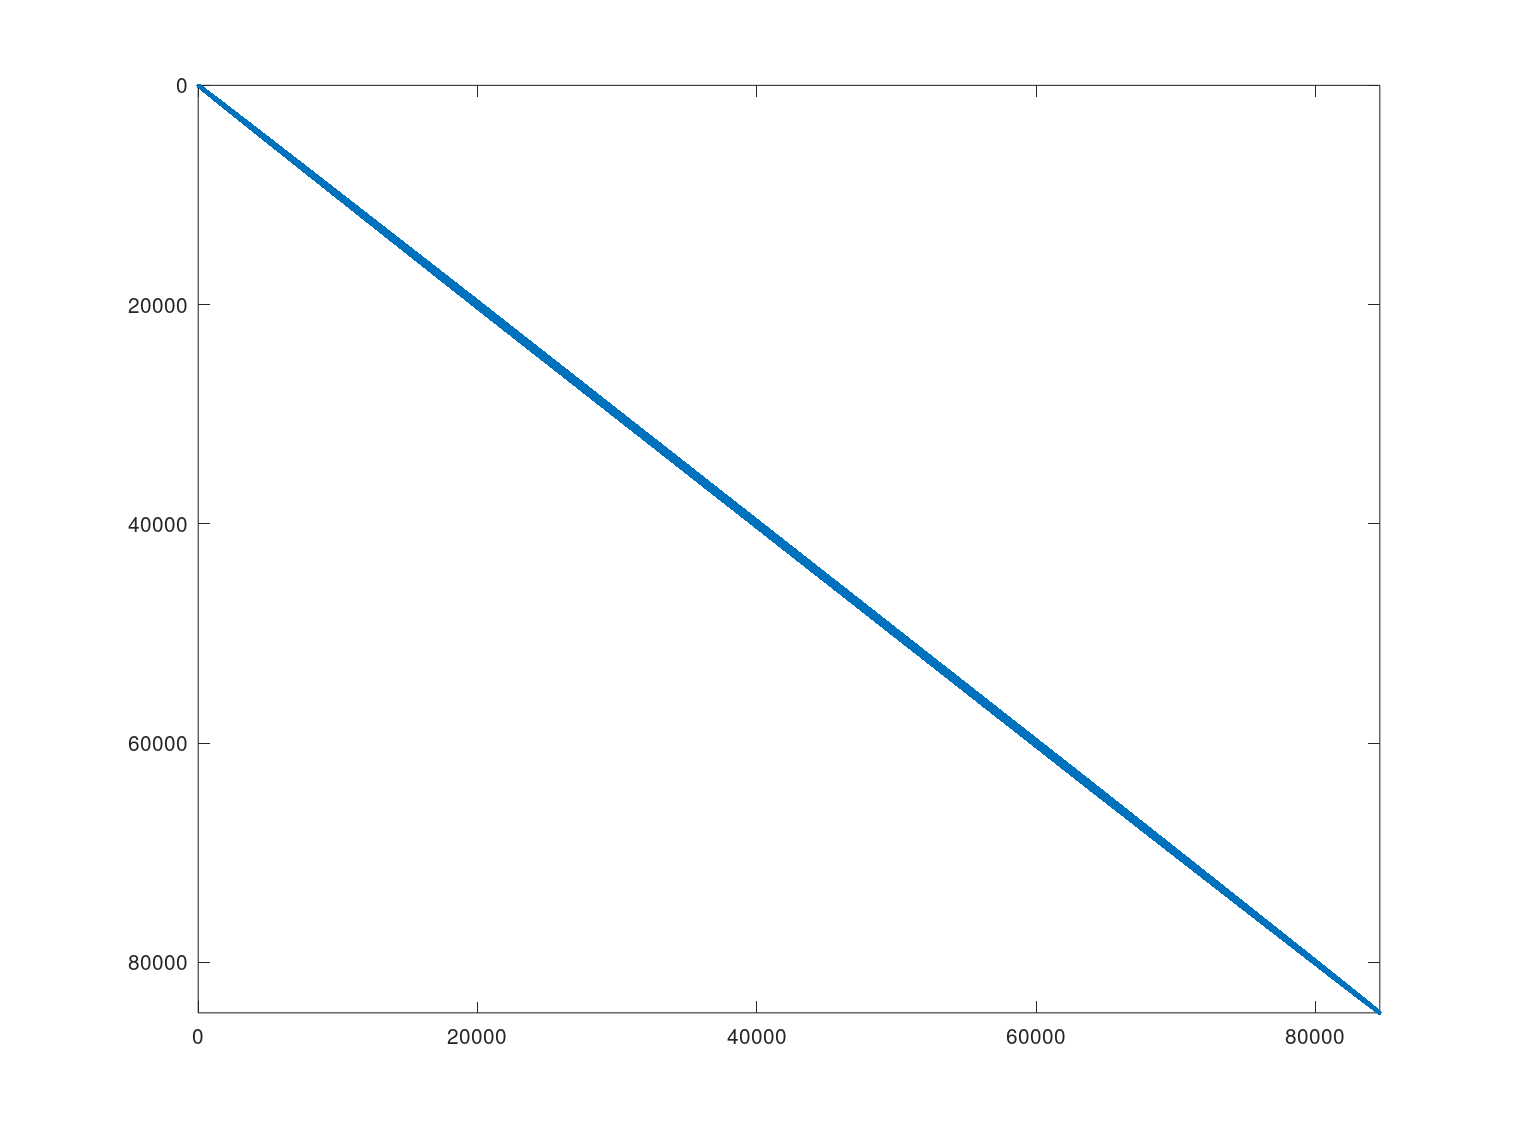
\includegraphics[width=\textwidth]{images/epb3_spyM_ILU_com.png}
         \caption{Spy após ILU com reordenamento}
         \label{fig:epb-ILU-c}
    \end{subfigure}
    \caption{Gráficos do preenchimento de \textit{epb3}.}
    \label{fig:epb}
\end{figure}

\section{Tabelas dos resultados observados}
\label{sec:tabelas}


\begin{table}[ht]
    \centering
    \begin{tabular}{|c|c|c|c|c|c|c|c|c|}
        \hline \rowcolor{Gray}
        \multicolumn{9}{|c|}{\bfseries Tabela de analise dos precondicionadores }\\
        \hline \rowcolor{Gray}  \multicolumn{4}{|c|}{} & \multicolumn{5}{|c|}{} \\
         [-1em]  \rowcolor{Gray}
         \multicolumn{4}{|c|}{\bfseries Informações da matriz } & \multicolumn{5}{|c|}{\bfseries Informações do precondicionamento }\\
         \hline \rowcolor{Gray} & & & & & & & &  \\
         [-1em]
         \rowcolor{Gray}
         \bfseries Nome & \bfseries n & \bfseries Não-nulos &  
         k = cond(A) & Precondicionador & Reordenamento &
         \bfseries Não-nulos &  
         k = cond(A)  & tempo (s) \\
         \hline \\
         [-1em] \bfseries mesh3em5 & 289 & 1377 & 4.965950e+00 & ICC(0) & com & 1889 & 4.965948e+00 & 0.000751972 s \\ & & & & & & & & \\ [-1em] \hline \\
         [-1em] \bfseries mesh3em5 & 289 & 1377 & 4.965950e+00 & ICC(0) & sem & 1891 & 4.965948e+00 & 0.000439167 s \\ & & & & & & & & \\ [-1em] \hline \\
         [-1em] \bfseries mesh3em5 & 289 & 1377 & 4.965950e+00 & ICC & com & 833 & 4.965944e+00 & 0.000847816 s \\ & & & & & & & & \\ [-1em] \hline \\
         [-1em] \bfseries mesh3em5 & 289 & 1377 & 4.965950e+00 & ICC & sem & 833 & 4.965944e+00 & 0.000476837 s \\ \hline
    \end{tabular}
    \caption{Tabela de análise dos precondicionadores utilizados na matriz \textit{mesh3em5}}
    \label{tab:precond-mesh}
\end{table}


\begin{table}[ht]
    \centering
    \begin{tabular}{|c|c|c|c|c|c|c|c|c|}
        \hline \rowcolor{Gray}
        \multicolumn{9}{|c|}{\bfseries Tabela do Método dos Gradientes Conjugados com tolerância $10^{-11}$ e máximo de iterações $10.000$ }\\
        \hline \rowcolor{Gray}  \multicolumn{2}{|c|}{} & \multicolumn{7}{|c|}{} \\
         [-1em]  \rowcolor{Gray}
         \multicolumn{2}{|c|}{\bfseries Informações da matriz } & \multicolumn{7}{|c|}{\bfseries Resultados do método }\\
         \hline \rowcolor{Gray} & & & & & & & & \\
         [-1em]
         \rowcolor{Gray}
         \bfseries Nome & \bfseries n & Precond. & Reordenamento & flag & iterações &
         erro relativo &
         $\|x\|_\infty$  & tempo (s) \\
         \hline & & & & & & & & \\
         [-1em] \bfseries mesh3em5 & 289 & - & -  & 0 & 20 & 6.495063e-12 & 1.000000e+00 & 0.00497293 s \\ & & & & & & &  \\ [-1em] \hline \\
         [-1em] \bfseries mesh3em5 & 289 & ICC(0) & com & 0 & 3 & 1.789972e-15 & 1.000000e+00 & 0.00606489 s \\ & & & & & & & & \\ [-1em] \hline \\
         [-1em] \bfseries mesh3em5 & 289 & ICC(0) & sem & 0 & 3 & 2.865405e-15 & 1.000000e+00 & 0.00613403 s \\ & & & & & & & & \\ [-1em] \hline \\
         [-1em] \bfseries mesh3em5 & 289 & ICC & com & 0 & 3 & 1.142175e-14 & 1.000000e+00 & 0.00574207 s \\ & & & & & & & & \\ [-1em] \hline \\
         [-1em] \bfseries mesh3em5 & 289 & ICC & sem & 0 & 3 & 1.142175e-14 & 1.000000e+00 & 0.00563097 s \\ \hline
    \end{tabular}
    \caption{Tabela de resultados observados na resolução da matriz \textit{mesh3em5} pelo Método Gradientes Conjugados com tolerância $10^{-11}$ e máximo de iterações $10.000$.}
    \label{tab:resultados-mesh}
\end{table}

\begin{table}[ht]
    \centering
    \begin{tabular}{|c|c|c|c|c|c|c|c|c|}
        \hline \rowcolor{Gray}
        \multicolumn{9}{|c|}{\bfseries Tabela de analise dos precondicionadores }\\
        \hline \rowcolor{Gray}  \multicolumn{4}{|c|}{} & \multicolumn{5}{|c|}{} \\
         [-1em]  \rowcolor{Gray}
         \multicolumn{4}{|c|}{\bfseries Informações da matriz } & \multicolumn{5}{|c|}{\bfseries Informações do precondicionamento }\\
         \hline \rowcolor{Gray} & & & & & & & &  \\
         [-1em]
         \rowcolor{Gray}
         \bfseries Nome & \bfseries n & \bfseries Não-nulos &  
         k = cond(A) & Precondicionador & Reordenamento &
         \bfseries Não-nulos &  
         k = cond(A)  & tempo (s) \\
         \hline \\
         [-1em] \bfseries 662\_bus & 662 & 2474 & 7.941311e+05 & ICC(0) & com & 2918 & 6.574479e+03 & 0.0118921 s \\ & & & & & & & & \\ [-1em] \hline \\
         [-1em] \bfseries 662\_bus & 662 & 2474 & 7.941311e+05 & ICC(0) & sem & 3702 & 5.903236e+03 & 0.000622034 s \\ & & & & & & & & \\ [-1em] \hline \\
         [-1em] \bfseries 662\_bus & 662 & 2474 & 7.941311e+05 & ICC & com & 4564 & 3.104181e+04 & 0.00163412 s \\ & & & & & & & & \\ [-1em] \hline \\
         [-1em] \bfseries 662\_bus & 662 & 2474 & 7.941311e+05 & ICC & sem & 5910 & 3.131869e+04 & 0.0014472 s \\ \hline
    \end{tabular}
    \caption{Tabela de análise dos precondicionadores utilizados na matriz \textit{662\_bus}}
    \label{tab:precond-bus}
\end{table}


\begin{table}[ht]
    \centering
    \begin{tabular}{|c|c|c|c|c|c|c|c|c|}
        \hline \rowcolor{Gray}
        \multicolumn{9}{|c|}{\bfseries Tabela do Método dos Gradientes Conjugados com tolerância $10^{-11}$ e máximo de iterações $10.000$ }\\
        \hline \rowcolor{Gray}  \multicolumn{2}{|c|}{} & \multicolumn{7}{|c|}{} \\
         [-1em]  \rowcolor{Gray}
         \multicolumn{2}{|c|}{\bfseries Informações da matriz } & \multicolumn{7}{|c|}{\bfseries Resultados do método }\\
         \hline \rowcolor{Gray} & & & & & & & & \\
         [-1em]
         \rowcolor{Gray}
         \bfseries Nome & \bfseries n & Precond. & Reordenamento & flag & iterações &
         erro relativo &
         $\|x\|_\infty$  & tempo (s) \\
         \hline & & & & & & & & \\
         [-1em] \bfseries 662\_bus & 662 & - & - & 0 & 678 & 8.627720e-11 & 1.000000e+00 & 0.100955 s \\ & & & & & & \\ [-1em] \hline \\
         [-1em] \bfseries 662\_bus & 662 & ICC(0) & com & 0 & 53 & 7.447388e-11 & 1.000000e+00 & 0.0568819 s \\ & & & & & & & & \\ [-1em] \hline \\
         [-1em] \bfseries 662\_bus & 662 & ICC(0) & sem & 0 & 76 & 7.837325e-11 & 1.000000e+00 & 0.0569861 s \\ & & & & & & & &  \\ [-1em] \hline \\
         [-1em] \bfseries 662\_bus & 662 & ICC & com & 0 & 10 & 9.035513e-12 & 1.000000e+00 & 0.0133121 s \\ & & & & & & & & \\ [-1em] \hline \\
         [-1em] \bfseries 662\_bus & 662 & ICC & sem & 0 & 10 & 6.091978e-12 & 1.000000e+00 & 0.014411 s \\ \hline
    \end{tabular}
    \caption{Tabela de resultados observados na resolução da matriz \textit{662\_bus} pelo Método Gradientes Conjugados com tolerância $10^{-11}$ e máximo de iterações $10.000$.}
    \label{tab:resultados-bus}
\end{table}

\begin{table}[ht]
    \centering
    \begin{tabular}{|c|c|c|c|c|c|c|c|c|}
        \hline \rowcolor{Gray}
        \multicolumn{9}{|c|}{\bfseries Tabela de analise dos precondicionadores }\\
        \hline \rowcolor{Gray}  \multicolumn{4}{|c|}{} & \multicolumn{5}{|c|}{} \\
         [-1em]  \rowcolor{Gray}
         \multicolumn{4}{|c|}{\bfseries Informações da matriz } & \multicolumn{5}{|c|}{\bfseries Informações do precondicionamento }\\
         \hline \rowcolor{Gray} & & & & & & & &  \\
         [-1em]
         \rowcolor{Gray}
         \bfseries Nome & \bfseries n & \bfseries Não-nulos &  
         k = cond(A) & Precondicionador & Reordenamento &
         \bfseries Não-nulos &  
         k = cond(A)  & tempo (s) \\
         \hline \\
         [-1em] \bfseries pdb1HYS & 36417 & 4344765 & -1.000000e+00 & ICC(0) & com & 9347919 & -1.000000e+00 & 2.12236 s \\ & & & & & & & & \\ [-1em] \hline \\
         [-1em] \bfseries pdb1HYS & 36417 & 4344765& -1.000000e+00 & ICC(0) & sem & 10409889 & -1.000000e+00 & 1.30761 s
         \\ \hline
    \end{tabular}
    \caption{Tabela de análise dos precondicionadores utilizados na matriz \textit{pdb1HYS}}
    \label{tab:precond-pdb}
\end{table}


\begin{table}[ht]
    \centering
    \begin{tabular}{|c|c|c|c|c|c|c|c|c|}
        \hline \rowcolor{Gray}
        \multicolumn{9}{|c|}{\bfseries Tabela do Método dos Gradientes Conjugados com tolerância $10^{-11}$ e máximo de iterações $10.000$ }\\
        \hline \rowcolor{Gray}  \multicolumn{2}{|c|}{} & \multicolumn{7}{|c|}{} \\
         [-1em]  \rowcolor{Gray}
         \multicolumn{2}{|c|}{\bfseries Informações da matriz } & \multicolumn{7}{|c|}{\bfseries Resultados do método }\\
         \hline \rowcolor{Gray} & & & & & & & & \\
         [-1em]
         \rowcolor{Gray}
         \bfseries Nome & \bfseries n & Precond. & Reordenamento & flag & iterações &
         erro relativo &
         $\|x\|_\infty$  & tempo (s) \\
         \hline & & & & & & & & \\
         [-1em] \bfseries pdb1HYS & 36417 & - & - & 3 & 6205 & 3.618273e-06 & 1.000001e+00 & 106.573 s \\ & & & & & & & &\\ [-1em] \hline \\
         [-1em] \bfseries pdb1HYS & 36417 & ICC(0) & com & 3 & 1026 & 8.864919e-07 & 1.000001e+00 & 3281.42 s \\ & & & & & & & & \\ [-1em] \hline \\
         [-1em] \bfseries pdb1HYS & 36417 & ICC(0) & sem & 3 & 1266 & 1.024893e-06 & 1.000001e+00 & 4548.05 s
         \\ \hline
    \end{tabular}
    \caption{Tabela de resultados observados na resolução da matriz \textit{pdb1HYS} pelo Método Gradientes Conjugados com tolerância $10^{-11}$ e máximo de iterações $10.000$.}
    \label{tab:resultados-pdb}
\end{table}

\begin{table}[ht]
    \centering
    \begin{tabular}{|c|c|c|c|c|c|c|c|c|}
        \hline \rowcolor{Gray}
        \multicolumn{9}{|c|}{\bfseries Tabela de analise dos precondicionadores }\\
        \hline \rowcolor{Gray}  \multicolumn{4}{|c|}{} & \multicolumn{5}{|c|}{} \\
         [-1em]  \rowcolor{Gray}
         \multicolumn{4}{|c|}{\bfseries Informações da matriz } & \multicolumn{5}{|c|}{\bfseries Informações do precondicionamento }\\
         \hline \rowcolor{Gray} & & & & & & & &  \\
         [-1em]
         \rowcolor{Gray}
         \bfseries Nome & \bfseries n & \bfseries Não-nulos &  
         k = cond(A) & Precondicionador & Reordenamento &
         \bfseries Não-nulos &  
         k = cond(A)  & tempo (s) \\
         \hline \\
         [-1em] \bfseries Dubcova3 & 146689 & 3636643 & - & ICC(0) & com & 4769297 & - & 0.913333 s \\ & & & & & & & & \\ [-1em] \hline \\
         [-1em] \bfseries Dubcova3 & 146689 & 3636643 & - & ICC(0) & sem & 16025173 & - & 1.03894 s \\ & & & & & & & & \\ [-1em] \hline \\
         [-1em] \bfseries Dubcova3 & 146689 & 3636643 & - & ICC & com & 8061119 & - & 1.71888 s \\ & & & & & & & & \\ [-1em] \hline \\
         [-1em] \bfseries Dubcova3 & 146689 & 3636643  & - & ICC & sem & 52898003 & - & 7.16305 s \\ \hline
    \end{tabular}
    \caption{Tabela de análise dos precondicionadores utilizados na matriz \textit{Dubcova3}}
    \label{tab:precond-Dub}
\end{table}


\begin{table}[ht]
    \centering
    \begin{tabular}{|c|c|c|c|c|c|c|c|c|}
        \hline \rowcolor{Gray}
        \multicolumn{9}{|c|}{\bfseries Tabela do Método Gradientes Conjugados com tolerância $10^{-11}$ e máximo de iterações $10.000$ }\\
        \hline \rowcolor{Gray}  \multicolumn{2}{|c|}{} & \multicolumn{7}{|c|}{} \\
         [-1em]  \rowcolor{Gray}
         \multicolumn{2}{|c|}{\bfseries Informações da matriz } & \multicolumn{7}{|c|}{\bfseries Resultados do método }\\
         \hline \rowcolor{Gray} & & & & & & & & \\
         [-1em]
         \rowcolor{Gray}
         \bfseries Nome & \bfseries n & Precond. & Reordenamento &  flag & iterações &
         erro relativo &
         $\|x\|_\infty$  & tempo (s) \\
         \hline & & & & & & & & \\
         [-1em] \bfseries Dubcova3 & 146689 & - & - & 0 & 215 & 9.438705e-11 & 1.000000e+00 & 4.30956 s \\ & & & & & & & &  \\ [-1em] \hline \\
         [-1em] \bfseries Dubcova3 & 146689 & ICC(0) & com & 0 & 97 & 9.742899e-11 & 1.000000e+00 & 299.55 s \\ & & & & & & & &  \\ [-1em] \hline \\
         [-1em] \bfseries Dubcova3 & 146689 & ICC(0) & sem & 0 & 143 & 9.606530e-11 & 1.000000e+00 & 1575.17 s \\ & & & & & & & & \\ [-1em] \hline \\
         [-1em] \bfseries Dubcova3 & 146689 & ICC & com & 0 & 26 & 2.954087e-11 & 1.000000e+00 & 138.95 s \\ & & & & & & & & \\ [-1em] \hline \\
         [-1em] \bfseries Dubcova3 & 146689 & ICC & sem & 0 & 32 & 6.821619e-11 & 1.000000e+00 & 1842 s \\ \hline
    \end{tabular}
    \caption{Tabela de resultados observados na resolução da matriz \textit{Dubcova3} pelo Método GMRES com tolerância $10^{-11}$ e máximo de iterações $10.000$.}
    \label{tab:resultados-Dub}
\end{table}

\begin{table}[ht]
    \centering
    \begin{tabular}{|c|c|c|c|c|c|c|c|c|}
        \hline \rowcolor{Gray}
        \multicolumn{9}{|c|}{\bfseries Tabela de analise dos precondicionadores }\\
        \hline \rowcolor{Gray}  \multicolumn{4}{|c|}{} & \multicolumn{5}{|c|}{} \\
         [-1em]  \rowcolor{Gray}
         \multicolumn{4}{|c|}{\bfseries Informações da matriz } & \multicolumn{5}{|c|}{\bfseries Informações do precondicionamento }\\
         \hline \rowcolor{Gray} & & & & & & & &  \\
         [-1em]
         \rowcolor{Gray}
         \bfseries Nome & \bfseries n & \bfseries Não-nulos &  
         k = cond(A) & Precondicionador & Reordenamento &
         \bfseries Não-nulos &  
         k = cond(A)  & tempo (s) \\
         \hline \\
         [-1em] \bfseries cavity05 & 1182 & 32632& 5.770648e+05 & ILU & sem & 133644 & 7.245709e+04 & 0.024977 s \\ \hline
    \end{tabular}
    \caption{Tabela de análise dos precondicionadores utilizados na matriz \textit{cavity05}}
    \label{tab:precond-cavity}
\end{table}


\begin{table}[ht]
    \centering
    \begin{tabular}{|c|c|c|c|c|c|c|c|c|c|}
        \hline \rowcolor{Gray}
        \multicolumn{10}{|c|}{\bfseries Tabela do Método GMRES com tolerância $10^{-11}$ e máximo de iterações $10.000$ }\\
        \hline \rowcolor{Gray}  \multicolumn{2}{|c|}{} & \multicolumn{8}{|c|}{} \\
         [-1em]  \rowcolor{Gray}
         \multicolumn{2}{|c|}{\bfseries Informações da matriz } & \multicolumn{8}{|c|}{\bfseries Resultados do método }\\
         \hline \rowcolor{Gray} & & & & & & & & & \\
         [-1em]
         \rowcolor{Gray}
         \bfseries Nome & \bfseries n & Precond. & Reordenamento & k & flag & iterações &
         erro relativo &
         $\|x\|_\infty$  & tempo (s) \\
         \hline & & & & & & & & & \\
         [-1em] \bfseries cavity05 & 1182 & - & - & 447 & 0 & 394 & 9.841954e-11 & 1.000001e+00 & 25.7365 s \\ & & & & & & & & \\ [-1em] \hline \\
         [-1em] \bfseries cavity05 & 1182 & ILU & sem & 447 & 0 & 27 & 6.987364e-11 & 1.000000e+00 & 2.76892 s\\ 
         \hline
    \end{tabular}
    \caption{Tabela de resultados observados na resolução da matriz \textit{cavity05} pelo Método GMRES com tolerância $10^{-11}$ e máximo de iterações $10.000$.}
    \label{tab:resultados-cavity}
\end{table}

\begin{table}[ht]
    \centering
    \begin{tabular}{|c|c|c|c|c|c|c|c|c|}
        \hline \rowcolor{Gray}
        \multicolumn{9}{|c|}{\bfseries Tabela de analise dos precondicionadores }\\
        \hline \rowcolor{Gray}  \multicolumn{4}{|c|}{} & \multicolumn{5}{|c|}{} \\
         [-1em]  \rowcolor{Gray}
         \multicolumn{4}{|c|}{\bfseries Informações da matriz } & \multicolumn{5}{|c|}{\bfseries Informações do precondicionamento }\\
         \hline \rowcolor{Gray} & & & & & & & &  \\
         [-1em]
         \rowcolor{Gray}
         \bfseries Nome & \bfseries n & \bfseries Não-nulos &  
         k = cond(A) & Precondicionador & Reordenamento &
         \bfseries Não-nulos &  
         k = cond(A)  & tempo (s) \\
         \hline \\
         [-1em] \bfseries cz2548 & 2548 & 25674  & 2.563753e+06 & ILU(0) & com & 33225  & 1.083267e+05 & 0.00527596 s \\ & & & & & & & &  \\ [-1em] \hline \\
         [-1em] \bfseries cz2548 & 2548 & 25674  & 2.563753e+06 & ILU(0) & sem & 36815  & 1.026009e+05 & 0.00266695 s \\ & & & & & & & &  \\ [-1em] \hline \\
         [-1em] \bfseries cz2548 & 2548 & 25674  & 2.563753e+06 & ILU & com & 25958  & 3.156199e+06 & 0.0166929 s \\ & & & & & & & &  \\ [-1em] \hline \\
         [-1em] \bfseries cz2548 & 2548 & 25674  & 2.563753e+06  & ILU & sem & 39000  & 3.479452e+05 & 0.0171821 s \\ \hline
    \end{tabular}
    \caption{Tabela de análise dos precondicionadores utilizados na matriz \textit{cz2548}}
    \label{tab:precond-cz}
\end{table}


\begin{table}[ht]
    \centering
    \begin{tabular}{|c|c|c|c|c|c|c|c|c|c|}
        \hline \rowcolor{Gray}
        \multicolumn{10}{|c|}{\bfseries Tabela do Método GMRES com tolerância $10^{-11}$ e máximo de iterações $10.000$ }\\
        \hline \rowcolor{Gray}  \multicolumn{2}{|c|}{} & \multicolumn{8}{|c|}{} \\
         [-1em]  \rowcolor{Gray}
         \multicolumn{2}{|c|}{\bfseries Informações da matriz } & \multicolumn{8}{|c|}{\bfseries Resultados do método }\\
         \hline \rowcolor{Gray} & & & & & & & & & \\
         [-1em]
         \rowcolor{Gray}
         \bfseries Nome & \bfseries n & Precond. & Reordenamento & k & flag & iterações &
         erro relativo &
         $\|x\|_\infty$  & tempo (s) \\
         \hline & & & & & & & & & \\
         [-1em] \bfseries cz2548 & 2548 & - & - & 760 & 0 & 1294 & 9.880078e-11 & 1.000000e+00 & 259.886 s \\ & & & & & & & & & \\ [-1em] \hline \\
         [-1em] \bfseries cz2548 & 2548 & ILU(0) & sem & 760 & 0 & 224 & 9.635935e-11 & 1.000000e+00 & 8.27269 s \\  & & & & & & & & & \\ [-1em] \hline \\
         [-1em] \bfseries cz2548 & 2548 & ILU(0) & com & 760 & 0 & 241 & 6.971360e-11 & 1.000000e+00 & 9.5068 s \\  & & & & & & & & & \\ [-1em] \hline \\
         [-1em] \bfseries cz2548 & 2548 & ILU & sem & 760 & 0 & 25 & 1.471816e-11 & 1.000000e+00 & 0.514301 s \\  & & & & & & & & & \\ [-1em] \hline \\
         [-1em] \bfseries cz2548 & 2548 & ILU & com & 760 & 0 & 16 & 4.466133e-12 & 1.000000e+00 & 0.219451 s \\ 
         \hline
    \end{tabular}
    \caption{Tabela de resultados observados na resolução da matriz \textit{cz2548} pelo Método GMRES com tolerância $10^{-11}$ e máximo de iterações $10.000$.}
    \label{tab:resultados-cz}
\end{table}

\begin{table}[ht]
    \centering
    \begin{tabular}{|c|c|c|c|c|c|c|c|c|}
        \hline \rowcolor{Gray}
        \multicolumn{9}{|c|}{\bfseries Tabela de analise dos precondicionadores }\\
        \hline \rowcolor{Gray}  \multicolumn{4}{|c|}{} & \multicolumn{5}{|c|}{} \\
         [-1em]  \rowcolor{Gray}
         \multicolumn{4}{|c|}{\bfseries Informações da matriz } & \multicolumn{5}{|c|}{\bfseries Informações do precondicionamento }\\
         \hline \rowcolor{Gray} & & & & & & & &  \\
         [-1em]
         \rowcolor{Gray}
         \bfseries Nome & \bfseries n & \bfseries Não-nulos &  
         k = cond(A) & Precondicionador & Reordenamento &
         \bfseries Não-nulos &  
         k = cond(A)  & tempo (s) \\
         \hline \\
         [-1em] \bfseries epb3 & 84617 & 463625 & -1.000000e+00 & ILU(0) & com & 565126 & -1.000000e+00 & 0.101275 s \\ & & & & & & & &  \\ [-1em] \hline \\
         [-1em] \bfseries epb3 & 84617 & 463625 & -1.000000e+00 & ILU(0) & sem & 571799 & -1.000000e+00 & 0.052027 s \\ & & & & & & & & \\ [-1em] \hline \\
         [-1em] \bfseries epb3 & 84617 & 463625 & -1.000000e+00 & ILU & com & 1500473 & -1.000000e+00 & 10.6831 s \\ & & & & & & & & \\ [-1em] \hline \\
         [-1em] \bfseries epb3 & 84617 & 463625 & -1.000000e+00 & ILU & sem & 1187509 & -1.000000e+00 & 10.1404 s \\ \hline
    \end{tabular}
    \caption{Tabela de análise dos precondicionadores utilizados na matriz \textit{epb3}}
    \label{tab:precond-epb}
\end{table}


\begin{table}[ht]
    \centering
    \begin{tabular}{|c|c|c|c|c|c|c|c|c|c|}
        \hline \rowcolor{Gray}
        \multicolumn{10}{|c|}{\bfseries Tabela do Método GMRES com tolerância $10^{-11}$ e máximo de iterações $10.000$ }\\
        \hline \rowcolor{Gray}  \multicolumn{2}{|c|}{} & \multicolumn{8}{|c|}{} \\
         [-1em]  \rowcolor{Gray}
         \multicolumn{2}{|c|}{\bfseries Informações da matriz } & \multicolumn{8}{|c|}{\bfseries Resultados do método }\\
         \hline \rowcolor{Gray} & & & & & & & & & \\
         [-1em]
         \rowcolor{Gray}
         \bfseries Nome & \bfseries n & Precond. & Reordenamento & k & flag & iterações &
         erro relativo &
         $\|x\|_\infty$  & tempo (s) \\
         \hline & & & & & & & & & \\
         [-1em] \bfseries epb3 & 84617 & - & - & 800 & 0 & 7411 & 9.991353e-11 & 1.000001e+00 & 3933.55 s \\ & & & & & & & & \\ [-1em] \hline \\
         [-1em] \bfseries epb3 & 84617 & ILU(0) & sem & 800 & 0 & 150 & 8.829092e-11 & 1.000000e+00 & 101.365 s \\ & & & & & & & & \\ [-1em] \hline \\
         [-1em] \bfseries epb3 & 84617 & ILU(0) & com & 800 & 0 & 185 & 9.210646e-11 & 1.000000e+00 & 174.184 s \\ & & & & & & & & \\ [-1em] \hline \\
         [-1em] \bfseries epb3 & 84617 & ILU & sem & 800 & 0 & 44 & 8.526528e-11 & 1.000000e+00 & 157.286 s \\ & & & & & & & & \\ [-1em] \hline \\
         [-1em] \bfseries epb3 & 84617 & ILU & com & 800 & 0 & 44 & 7.579705e-11 & 1.000000e+00 & 209.548 s \\ \hline
    \end{tabular}
    \caption{Tabela de resultados observados na resolução da matriz \textit{epb3} pelo Método GMRES com tolerância $10^{-11}$ e máximo de iterações $10.000$.}
    \label{tab:resultados-epb}
\end{table}

\clearpage
\normalsetting

\end{document}
